\newpage 

% 
% Introduction of the BLSM.  
% 
% 

%\section{B-L-SM Model}
\chapter{B-L-SM Model} 
\label{Chap:B-L-SM_Model}

% Got this from the abstract in my BLSM paper 

%Here we start the our first look at BSM scenarios. 
%
In this chapter we introduce the minimal $\U{B-L}$ gauge extension of the SM named, the B-L-SM (Baryon-Lepton-SM) Model \cite{Mohapatra:1980qe,Basso:2010hk,Basso:2011na}. 
%
In this model, we are capable of explaining the generation of neutrinos masses generation via a simple see-saw mechanism. Additionally, by virtue of two new physical states, specifically a new Higgs like boson $\mathrm{H}^\prime$ and a $\mathrm{Z}^\prime$ gauge boson we can also address other phenomenology, such as deviations in EW measurements, namely the $(g-2)_\mu$ anomaly \cite{Tanabashi:2018oca}. 

The additional bosons aquire mass primarily trough the spontaneous breaking of the $\U{B-L}$ symmetry that gives it's name to the model.
%
This unitary group originates from the promotion of an accidental symmetry present in the SM, the Baryon number (B) minus the Lepton number (L) to a fundamental Abelian symmetry group. 
%
This origin for the mass of the referenced bosons means the model is already very heavily constrained due to long-standing direct searches at the LHC. 

Through this model we can address the metastability of the EW vacuum in the SM trough the new scalar. Allowing for Higgs stabilization up to the Plank scale with a new Higgs starting from a few hundred GeVs \cite{Degrassi:2012ry,Alekhin:2012py,Buttazzo:2013uya}. 

The B-L-SM framework is particular interesting in the context of the study of Grand Unified Theories (GUT) as it easily embedded into higher order symmetry groups like the $\mathrm{SO(10)}$ \cite{Chanowitz:1977ye,Fritzsch:1974nn,Georgi:1978fu,Georgi:1979dq,Georgi:1979ga} or $\mathrm{E}_6$ \cite{Achiman:1978vg,Gursey:1975ki,Gursey:1981kf} Lie groups.   
The presence of a new complex singlet field, $\chi$, with a Higgs doublet typically results in enhanced strength of the EW phase transition potentially converting it into a strong first-order one. This would be could be detectable in the form of a gravitational wave background \cite{Barger:2008jx}. 
%
Such a analysis is of utmost importance given that it could provide a way to detect NP or exclude models without the need for a larger particle collider. % but instead a sensitive probe also capable of studying gravitational events. 

However, a family-universal symmetry such as $\mathrm{U(1)_{B-L}}$, being introduced without changing the SM fermion content would lead to chiral anomalies. This translates to a non conservative charged current on some channels involving the $\mathrm{U(1)_{B-L}}$. These are not completely undesired by themselves, as they would allow for the presence of extra sources of $\mathcal{CP}$ violation, but this inclusion at tree-level without a suppression mechanism would lead to far too much $\mathcal{CP}$ violation. 

The model also benefits from the presence of three generations of right-handed heavy Majorana neutrinos that through the new field additions are possible in a framework free of anomalies while also allowing for a minimal see-saw mechanism that generates light neutrino masses unlike the SM.  \cite{Yanagida:1979as,GellMann:1980vs,Mohapatra:1979ia}.´
%
The mass scale of such neutrinos is established once the $\U{B-L}$ symmetry is broken. 
%
These neutrinos are of cosmological significance given their presence could imply the existence of a sterile state that can play the role of Dark Matter \cite{Kaneta:2016vkq}.
%
The relatively small alteration of a, $\mathbb{Z}_2$, symmetry in the neutrino sector can make these fully sterile, as seen in \cite{Okada:2010wd,Okada:2018ktp}. {\color{red} Check if the Z2 affects the Zprime, if so we must comment that it doens't allow kinetic mixing! and would alter the $a_\mu$. Acho que não. Não deve haver alterações dos couplings com o muão, portanto a um loop não acontece nada. A dois loops, também não deve haver, pois os neutrinos não tem carga e não acoplam ao fotão, dos diagramas que aparecem na Fig. 4.7 Preciso mesmo de falar com o morais para ter a certeza.}
%
These neutrinos can, in such case, be used to help explain the baryon asymmetry via the leptogenesis mechanism, this scenario is discussed in depth in the following Refs.~\cite{Fukugita:1986hr,Pilaftsis:1997jf,Pilaftsis:2003gt}. 

With this in mind, we structure this chapter in the fol-
lowing way. First, we present the fundamental theoretical background on the model with a strong focus on the basic details of the scalar and the gauge boson mass spectra and mixing. Followed by a modern precise study of the phenomenological status of the B-L-SM model trough a layered algorithm that will be discussed preceding the results. With this algorithm we provide a numerical analysis that tests the relevant phenomenological constraints in direct and EW observables. FFollowed by this study, we table off a few representative benchmark points. 

% { \color{blue} perhaps I should include this on the start of the chapter  }

\section{Formulating the model}

Essentially, the minimal B-L-SM is a BSM framework containing only three new ingredients, a new gauge interaction given the new symmetry group, three generations of right handed neutrinos, and a complex scalar field $\chi$. 

The first of these is well motivated by the aformentioned GUT scenarios, While a new sector of additional three $\mathrm{U(1)_{B-L}}$ charged Majorana neutrinos is essential for anomaly cancellation.
%The first of these, is motivated by the aforementioned GUT scenarios, as seen in the Refs, \cite{Chanowitz:1977ye,Fritzsch:1974nn,Georgi:1978fu,Georgi:1979dq,Georgi:1979ga,Achiman:1978vg,Gursey:1975ki,Gursey:1981kf}, here you can see that the B-L-SM can be introduced in a large number of groups, like $E_6$ and $\mathrm{SO}(10)$. 
%
%Secondly, as mentioned, a new sector of additional three $U(1)_{B-L}$ charged Majorana neutrinos is essential for anomaly cancellation and addresses many concerns of the SM. 

Finally, the SM-like Higgs doublet, $H$, does not carry neither baryon nor lepton number, this way it does not participate in the breaking of $\mathrm{U(1)_{B-L}}$. It is then necessary to introduce a new scalar singlet field, $\chi$, solely charged under $\mathrm{U(1)_{B-L}}$, to perform the breaking of the $\mathrm{B-L}$ symmetry.

The particle content and related charges of the minimal $U(1)_{B-L}$ extension of the SM are shown in Tab \ref{tab:BLSM_Charges}. Note these are similar to the SM as to be expected. 
%
\begin{table}[H]
\centering
\begin{tabular}{|c|c|c|c|c|c|c|c|c|}
\hline
  & $q_L$  & $u_R$ & $d_R$ & $l_L$  & $e_R$ & $\nu_R$  &  $H$  & $\chi$  \\ \hline
 $\mathrm{SU(3)_C}$& $\mathbf{3}$ & $\mathbf{3}$  & $\mathbf{3}$  & $\mathbf{1}$  & $\mathbf{1}$   & $\mathbf{1}$   & $\mathbf{1}$    & $\mathbf{1}$    \\
 $\mathrm{SU(2)_L}$& $\mathbf{2}$  & $\mathbf{1}$ & $\mathbf{1}$ & $\mathbf{2}$ & $\mathbf{1}$ & $\mathbf{1}$ & $\mathbf{2}$  & $\mathbf{1}$ \\
$\mathrm{U(1)_Y}$ & ${1}/{6}$ & ${2}/{3}$  & -${1}/{3}$  & -${1}/{2}$ & -1 & 0 & ${1}/{2}$ & 0 \\
$\mathrm{U(1)_{B-L}}$ & ${1}/{3}$ & ${1}/{3}$ & ${1}/{3}$  & -1  & -1 &-1  & 0 & 2  \\ \hline 
\end{tabular}
\caption{Quantum fields and their respective quantum numbers in the minimal B-L-SM extension. The last two lines represent the weak and $B-L$ hypercharges}
\label{tab:BLSM_Charges}
\end{table} 

\subsubsection{Scalar sector}

With the information from Tab \ref{tab:BLSM_Charges}, we can begin examining the new Lagrangian terms. Starting by the scalar potential, which now depends on two fields, 
%
\begin{equation}
\label{eq:potential}
V(H,\chi) = \mu_1^2 H^\dagger H + \mu_2^2 \chi^\ast \chi + \lambda_1 (H^\dagger H)^2 + \lambda_2 \left(\chi^\ast \chi\right)^2 + \lambda_3  \chi^\ast \chi H^\dagger H , 
\end{equation}
%
where,  $\lambda_i$, the scalar couplings and $\mu_{1,2}^2$ the quadratic terms for $H$ and $\chi$ respectively. This potential must lead to a stable vacuum state, which means that the scalar potential must be bounded from below (BFB), as to ensure a global minima.  Studying the potential on Eq.\,(\ref{eq:potential}) we deduce the conditions,
\begin{equation}
4 \lambda_1 \lambda_2  -  \lambda_3^2 > 0 \quad , \quad \lambda_1 , \lambda_2>0 
\label{eq:BFB}
\end{equation}
%
Where the full components of the scalar fields $H$ and $\chi$ are given by,
\begin{equation}
H = \frac{1}{\sqrt{2}} 
\begin{pmatrix}
-i \( \omega_1 - i \omega_2 \) \\
v + (h + i z)
\end{pmatrix} \quad \chi = \frac{1}{\sqrt{2}} \( x + \(h^\prime + i z^\prime\) \)
\end{equation}
%
where we note that the parameters $v$ and $x$ are VEV’s associated with the $H$ field and the $\chi$ field, respectively.
In these equations we can see that $h$ and $h^\prime$ represent the radial quantum fluctuations around the minimum of the potential. These will constitute the physical degrees of freedom associated with $H$ and $H^\prime$. There are also four Goldstone directions denoted as $\omega_1$, $\omega_2$, $z$ and $z^\prime$ which are absorbed into longitudinal modes of the $W^\pm$, $Z$ and $Z^\prime$ gauge bosons once SSB takes place. After SSB the associated VEVs take the form, 
%
\begin{equation}
 \langle H \rangle = \frac{1}{\sqrt{2}} 
\begin{pmatrix}
0 \\
v 
\end{pmatrix}	
\qquad
 \langle  \chi \rangle  = \frac{x}{\sqrt{2}}
\label{eq:vacuum}
\end{equation}
% 
%here, recall $v$ and $x$ are the associated VEVs to each field. 
From here we can solve the tadpole equations in relation to each of the VEVs as to ensure non-zero VEV. We arrive at,
%
\begin{equation}
	v^2 = \tfrac{-\lambda_2 \mu_1^2 + \tfrac{\lambda_3}{2}\mu_2^2}{\lambda_1 \lambda_2 - \tfrac{1}{4}\lambda_3^2} > 0
	\qquad
	\text{and}
	\qquad
	x^2 = \tfrac{-\lambda_1 \mu_2^2 + \tfrac{\lambda_3}{2}\mu_1^2}{\lambda_1 \lambda_2 - \tfrac{1}{4}\lambda_3^2} > 0 
	\label{eq:extremum}
\end{equation}
%
which, when simplified with the BFB conditions yield a simpler set of equations,
%
\begin{equation}
\lambda_2 \mu_1^2 < \tfrac{\lambda_3}{2} \mu_2^2 
\qquad
\text{and}
\qquad
\lambda_1 \mu_2^2 < \tfrac{\lambda_3}{2} \mu_1^2
\label{eq:sols}
\end{equation}
%
Note that although $\lambda_1$ and $\lambda_2$ must be positive to ensure the correct conical shape of the potential, no such conditions exist for the sign of $\lambda_3$ , $\mu_1$, and $\mu_2$. However observing Eq\,(\ref{eq:sols}) we can infer that only some combinations of signs are impossible, 
%
\begin{table}[H]
	\begin{center}
		\begin{tabular}{ccccc}
			& $\mu_2^2 > 0$ & $\mu_2^2 > 0$ & $\mu_2^2 < 0$ & $\mu_2^2 < 0$  	\\
			& $\mu_1^2 > 0$ & $\mu_1^2 < 0$ & $\mu_1^2 > 0$ & $\mu_1^2 < 0$  	\\        
			\hline  
			$\lambda_3 < 0 $     			    							& \xmark		& \checkmark	&	\checkmark & \checkmark	\\
			$\lambda_3 > 0$     			    							& \xmark		& \xmark	&	\xmark &  \checkmark \\
			\hline
		\end{tabular} 
		\caption{Possible signs of the potential parameters in Eq\,(\ref{eq:potential}). 
The \checkmark\,symbol indicates the existence of solutions for tadpole conditions Eq.\,(\eqref{eq:sols}), while the \xmark\,indicates unstable configurations.}
		\label{tab:signs}  
	\end{center}
\end{table} 
%
For our numerical analysis we decided to leave the sign of $\lambda_3$ positive, choosing a configuration where both $\mu$ parameters are negative. 
%
This does not directly translate to any real physical consequence.  
%
With these conditions now established we proceed to investigate the physical states of the B-L-SM scalar sector. 
%
At the vacuum, we evaluate the Hessian matrix as,
%
\begin{equation}
\mathbf{M}^2 =
\begin{pmatrix}
4 \lambda_2 x^2 & \lambda_3 v x \\ 
\lambda_3 v x   & 4 \lambda_1 v^2 
\end{pmatrix}\,,
\label{eq:hess}
\end{equation}
% 
Moving this matrix to its physical mass eigen-base, we obtain the following eigenvalues,
%
\begin{equation}
m_{h_{1,2}}^2 = \lambda_1 v^2 + \lambda_2 x^2 \mp \sqrt{(\lambda_1 v^2 - \lambda_2 x^2)^2 + (\lambda_3 x v)^2}.
\label{eq:eigvals}
\end{equation}
The physical basis vectors $h_1$ and $h_2$ can then be related to the original fields of gauge eigen-basis $h$ and $h^\prime$ trough a simple rotation matrix:
%
\begin{equation}
	\begin{pmatrix}
	h_1 \\
	h_2 
	\end{pmatrix}
	=
	\mathbf{O}
	\begin{pmatrix}
	h \\
	h^\prime 
	\end{pmatrix},
	\label{eq:trans}
\end{equation}
%
where $\mathbf{O}$ can be parameterized by a single mixing angle $\alpha_h$,
%
\begin{equation}
	\mathbf{O} = 
	\begin{pmatrix}
	\cos \alpha_h & -\sin \alpha_h \\
	\sin \alpha_h & \cos \alpha_h 
	\end{pmatrix}\,.
	\label{eq:rotmat}
\end{equation}
%
The precise mixing angle is represented simply by, 
\begin{equation}
\tan 2 \alpha_h   = \frac{ \left| \lambda_3 \right|  v x }{  \lambda_2 x^2 -\lambda_1 v^2 } 
\end{equation} 
%
It is particularly interesting to analyse the scenario where the scalar fields approximately decouple, that is, in the limit, $v/x\ll 1$. In these circumstances, the scalar masses and the mixing angle become rather simple,
\begin{equation}
\sin \alpha_h \approx \dfrac{1}{2}\dfrac{\lambda_3}{\lambda_2} \dfrac{v}{x} \qquad
m_{h_1}^2 \approx 2 \lambda_1 v^2 \qquad m_{h_2}^2 \approx 2 \lambda_2 x^2
\label{eq:simplify}
\end{equation}
%
We will see in the context of our numerical results that for a phenomenologically consistent mass scale these equations serve as a valid approximation for most of the  points. 

\subsubsection{Gauge Sector}

Moving onto the gauge boson and Higgs kinetic terms in the B-L-SM, consider the following portion of the Lagrangian,
\begin{equation}
\mathcal{L}_{\mathrm{U(1)'s}} =  \left| D_\mu H \right|^2 + \left| D_\mu \chi \right|^2 -\dfrac{1}{4} F_{\mu \nu} F^{\mu \nu} -\dfrac{1}{4} F^\prime_{\mu \nu} F^{\prime \mu \nu} -\dfrac{1}{2} \kappa F_{\mu \nu} F^{\prime \mu \nu}
\label{eq:Lu1}
\end{equation}
where $F^{\mu \nu}$ and $F^{\prime \mu \nu}$ are the standard field strength tensors, respectively for the $\U{Y}$ and  $\U{B-L}$ Abelian groups, 
\begin{equation}
	F_{\mu \nu} = \partial_\mu A_\nu - \partial_\nu A_\mu 
	\qquad
	\text{and}
	\qquad
	 F^\prime_{\mu \nu} = \partial_\mu A^\prime_\nu - \partial_\nu A^\prime_\mu\,.
	 \label{eq:Fmn}
\end{equation}
written in terms of the gauge fields $A_\mu$ and $A_\mu^\prime$, respectively. Given that this is a model with two Unitary groups, without a parity symmetry ($\mathbb{Z}_2$) to prevent it, we must consider the possible mixing in between them. In this work we parameterized this mixing trough a parameter $\kappa$.

The Abelian part of the covariant derivative in Eq.\,( \ref{eq:Lu1}) is given by,
\begin{equation}
	D_\mu \supset i g_1 Y A_\mu + i g_1^\prime Y_{\rm B-L} A_\mu^\prime\,,
\end{equation} 
% 
with $g_1$ and $g_1^\prime$ the $\U{Y}$ and $\U{B-L}$ the gauge couplings with the $Y$ and $B-L$ charges are specified in Tab.~\ref{tab:charges}. It is convenient to rewrite the gauge kinetic terms in the canonical form, i.e.
%
\begin{equation}
	F_{\mu \nu} F^{\mu \nu} + F^\prime_{\mu \nu} F^{\prime \mu \nu} + 2 \kappa F_{\mu \nu} F^{\prime \mu \nu} \to B_{\mu \nu} B^{\mu \nu} + B^\prime_{\mu \nu} B^{\prime \mu \nu}\,.
	\label{eq:AtoB}
\end{equation}
%
A generic orthogonal transformation in the field space does not eliminate the kinetic mixing term. So, in order to satisfy Eq.~\eqref{eq:AtoB} an extra non-orthogonal transformation should be imposed such that Eq.~\eqref{eq:AtoB} is realized. Taking $\kappa = \sin \alpha$, a suitable redefinition of fields $\{A_\mu,A_\mu^\prime\}$ into $\{B_\mu, B_\mu^\prime\}$ that eliminates $\kappa$-term according to Eq.~\eqref{eq:Lu1} can be cast as
\begin{equation}
	\begin{pmatrix}
	A_\mu \\
	A^\prime_\mu 
	\end{pmatrix}
	=
	\begin{pmatrix}
	1 & -\tan \alpha \\
	0 & \sec \alpha 
	\end{pmatrix}
	\begin{pmatrix}
	B_\mu \\
	B^\prime_\mu 
	\end{pmatrix}\,,
	\label{eq:trans-kappa}
\end{equation}
Note there is a limit without kinetic mixing where $\alpha = 0$. Note that this transformation is generic and valid for any basis in the field space. The transformation (\ref{eq:trans-kappa}) results in a modification of the covariant derivative that acquires two additional terms encoding the details of the kinetic mixing, i.e.

\begin{equation}
D_\mu \supset \partial_\mu + i \(g_Y \; Y + g_BY \; Y_{B-L}\) B_\mu + i \(g_{B-L} \; Y_{B-L} + g_{YB} \; Y\) B_\mu^\prime\,,
\label{eq:newCov}
\end{equation}	
where the gauge couplings take the form
\begin{equation}
	\begin{cases}
	g_Y = g_1 \\
	g_{B-L} = g_1^\prime \sec \alpha \\
	g_{YB} = -g_1 \tan \alpha \\
	g_{BY} = 0
	\end{cases} \,,
	\label{eq:new-g-simp}
\end{equation}
which is the standard convention in the literature. Note that this definition is merely to simplify the equations and has no physical impact. We will later see that this kinetic mixing is a desired feature and why stabilizing it with a $\mathbb{Z_2}$ symmetry would be detrimental in terms of depth. The resulting mixing between the neutral gauge fields including $Z^\prime$ can be represented as follows
%
\begin{equation}
\begin{aligned}
\begin{pmatrix}
\gamma_\mu \\
Z_\mu \\
Z^\prime_\mu
\end{pmatrix}
=
\begin{pmatrix}
\cos \theta_W & \sin \theta_W & 0\\
-\sin \theta_W \cos \theta_W^\prime & \cos \theta_W \cos \theta_W^\prime & \sin \theta_W^\prime \\
\sin \theta_W \sin \theta_W^\prime & -\cos \theta_W^\prime \sin \theta_W^\prime & \cos \theta_W^\prime
\end{pmatrix}
\begin{pmatrix}
B_\mu \\
A^3_\mu \\
B^\prime_\mu
\end{pmatrix}
\end{aligned}
\label{eq:g-Z-Zp}
\end{equation}	
%
where $\theta_W$ is the weak mixing angle and $\theta^\prime_W$ is defined as
\begin{equation}
\sin(2 \theta^\prime_W) = \frac{2 g_{YB} \sqrt{g^2 + g_{Y}^2}}{\sqrt{(g_{YB}^2 + 16 (\frac{x}{v})^2 g_{B-L}^2 - g^2 - g_{Y}^2)^2 + 4 g_{YB}^2 (g^2 + g_{Y}^2)} }\,,
\label{eq:theta-p-full}
\end{equation}
%
in terms of $g$ and $g_{Y}$ being the $\mathrm{SU(2)_{L}}$ and $\mathrm{U_{Y}}$ gauge couplings, respectively. In the physically relevant limit, $v/x \ll 1$, the above expression greatly simplifies leading to
%
\begin{equation}
	\sin \theta_W^\prime \approx \dfrac{1}{16
	} \dfrac{g_{YB}}{g_{B-L}}\( \dfrac{v}{x} \)^2 \sqrt{g^2 + g_{Y}^2} \,,
	\label{eq:theta-p}
\end{equation}
%
up to $(v/x)^3$ corrections. In the limit of no kinetic mixing, i.e. $g_{YB} \to 0$, there is no mixture of $Z^\prime$ and SM gauge bosons. 

Note, that the kinetic mixing parameter $\theta_W^\prime$ has rather stringent constraints from $Z$ pole experiments both at the Large Electron-Positron Collider (LEP) and the Stanford Linear Collider (SLC), restricting its value to be smaller than $10^{-3}$ approximately \cite{Bandyopadhyay_2018}, which we set as an upper bound in our numerical analysis. Expanding the kinetic terms $\left| D_\mu H \right|^2 + \left| D_\mu \chi \right|^2$ around the vacuum one can extract the following mass matrix for the vector bosons
\begin{equation}
	m_V^2 =
	\dfrac{v^2}{4}
	\begin{pmatrix}
	g^2 \;\;&\;\; 0 \;\;&\;\; 0 \;\;&\;\; 0 \;\;&\;\; 0 \\
	0 \;\;&\;\; g^2 \;\;&\;\; 0 \;\;&\;\; 0 \;\;&\;\; 0 \\
	0 \;\;&\;\; 0 \;\;&\;\; g^2 \;\;&\;\; -g g_{Y} \;\;&\;\; -g g_{YB} \\
	0 \;\;&\;\; 0 \;\;&\;\; -g g_{Y} \;\;&\;\; g_{Y}^2 \;\;&\;\; g_{Y} g_{YB} \\
	0 \;\;&\;\; 0 \;\;&\;\; -g g_{YB} \;\;&\;\; g_{Y} g_{YB} \;\;&\;\; g_{YB}^2 + 16 \(\dfrac{x}{v}\)^2 g_{B-L}^2
	\end{pmatrix}
\end{equation}
%
whose, first set of eigenvalues read,
\begin{equation}
	m_A = 0 \, \text{,} \qquad m_W = \tfrac{1}{2} v g
\end{equation}
corresponding to the expected physical photon and $W^\pm$ bosons. While the following set,
\begin{equation}
m_{Z,Z^\prime}=\sqrt{g^2 + g^2_{Y}} \cdot \frac{v}{2}  \sqrt{\frac{1}{2} \left( \frac{g_{YB}^2 + 16 (\frac{x}{v})^2 g^2_{\rm BL} }{g^2 + g^2_{\rm Y}} +1  \right) \mp \frac{g_{YB}}{\sin(2 \theta_W^\prime) \sqrt{g^2 + g^2_{\rm Y}}}}\,.
\label{eq:ZZp-mass}
\end{equation}
correspond to two neutral massive vector bosons, with one of them, not necessarily the lightest, representing the SM-like $Z$ boson. It follows from LEP and SLC constraints on $\theta_W^\prime$, that Eq.~\eqref{eq:theta-p} also implies that either $g_{YB}$ or the ratio ${v}/{x}$ are small. In this limit, Eq.~\eqref{eq:ZZp-mass} simplifies to
\begin{equation}
	m_Z \approx \tfrac{1}{2} v \sqrt{g^2 + g_{Y}^2} \qquad \text{and} \qquad m_{Z^\prime} \approx 2 g_{B-L} x\,,
	\label{eq:mZ}
\end{equation}
%
where the $m_{Z^\prime}$ depends only on the SM-singlet VEV ,$x$ and on the $\mathrm{U(1)_{B-L}}$ gauge coupling and will be attributed to a heavy $Z^\prime$ state, while the light $Z$-boson mass corresponds to its SM value.

\subsubsection{The Yukawa sector}

One of the key features of the B-L-SM model is the presence of non-zero neutrino masses. In its minimal version, such masses are generated via a type-I seesaw mechanism, thus producing a very light neutrino for each of the three known neutrino flavours, and a corresponding heavy neutrino one for each, which has yet to be observed. In the type-I seesaw mechanism the mixing of neutrinos fields is written with similar shape to, 
\begin{equation}
\left( \begin{array}{c|c}
0 & A \\
\midrule
A & B 
\end{array} \right) 
\end{equation}
This system would have a set eigenvalues written as, 
\begin{equation}
\lambda_\pm = \frac{ B \pm \sqrt{B^2 + 4 A} }{ 2 } 
\end{equation}
Investigating the nature of this set of eigenvalues allows us to understand the see-saw process. The mean of these values being always equal to $|B|$, if one value goes up, another goes down, like a see-saw. $B$ is set to be proportional to Majorana mass terms, orders of magnitude higher than the cross-terms $A$. Given this, the smaller eigenvalue, is, 
\begin{equation}
\lambda_- \approx \frac{A^2}{B}
\end{equation}
This mechanism serves to explain why the neutrino masses are so small. 

The total Yukawa Lagrangian of the model reads,
\begin{equation}
\begin{aligned}
\mathcal{L}_f = 
-Y_u^{ij} \bar{q}_{\rm L i} u_{\rm R j} \widetilde{H} 
-Y_d^{ij} \bar{q}_{\rm L i} d_{\rm R j} H
-Y_e^{ij} \bar{\ell}_{\rm L i} e_{\rm R j} H
- Y_\nu^{ij} \bar{\ell}_{\rm L i} \nu_{\rm R j} \widetilde{H}
	-\dfrac{1}{2} Y_\chi^{ij} \overline{\nu}_{\rm R i}^c \nu_{\rm R j} \chi + {\rm H.c.}
\end{aligned}
\label{eq:Yuk}
\end{equation}
%
Notice the explicit lack of Majorana neutrino mass terms of the form $M \overline{\nu_{R}^c} \nu_{R}$. These explicitly violate the $\mathrm{U(1)_{B-L}}$ symmetry and are therefore not present. In Eq.~\eqref{eq:Yuk}, $Y_u$, $Y_d$ and $Y_e$ are the $3 \times 3$ Yukawa matrices that reproduce the quark and charged lepton sector exactly the same way as in the SM, while $Y_\nu$ and $Y_\chi$ are the new Yukawa matrices responsible for the generation of right handed neutrino masses and mixing with left handed fields. In particular, one can write,
\begin{equation}
	\mathbf{m}_{\nu_l}^{Type-I} = \dfrac{1}{\sqrt{2}}\dfrac{v^2}{x} \mathbf{Y}_\nu^t \mathbf{Y}^{-1}_\chi \mathbf{Y}_\nu\,,
\end{equation}
%
for light $\nu_l$ neutrino masses, whereas the heavy $\nu_h$ ones are given by
\begin{equation}
	\mathbf{m}_{\nu_h}^{Type-I} \approx \dfrac{1}{\sqrt{2}} \mathbf{Y}_\chi x\,,
\end{equation} 
where we have assumed a flavour diagonal basis.

Note that the smallness of light neutrino masses imply that either the $x$ VEV is very large or (if we fix it to be at the $\mathcal{O}\left({\mathrm{TeV}}\right)$ scale and $\mathbf{Y}_\chi \sim \mathcal{O}\(1\right)$) the corresponding Yukawa coupling should be tiny, $\mathbf{Y}_\nu < 10^{-6}$. It is clear that the low scale character of the type-I seesaw mechanism in the minimal B-L-SM is \textit{faked} by small Yukawa couplings to the Higgs boson. A more elegant description was proposed in Ref.~\cite{Khalil:2010iu} where small SM neutrino masses naturally result from an inverse seesaw mechanism. In this work, however, we will not study the neutrino sector and thus, for an improved efficiency of our numerical analysis of $Z^\prime$ observables, it will be sufficient to fix the Yukawa couplings to $\mathbf{Y}_\chi = 10^{-1}$ and $\mathbf{Y}_\nu = 10^{-7}$ values such that the three lightest neutrinos lie in the sub-eV domain.


%\subsubsection{Neutrino masses}

%As mentioned briefly during the course of this dissertation the SM suffers from lacking a way to explain the observed neutrino masses by default. The minimal way of addressing this problem is by adding heavy Majorana type neutrinos in order to realise a seesaw mechanism. In this chapter we hope to explain how by perform the addition we could generate light neutrino states and how this addition is justified as part of a larger theory. 

% Explaining the seesaw. 

\section{Numerical Results}

Before we begin this section, we would like to point-out recent work done by our colleges where a comprehensive study for the $Z^\prime$ at the LHC is performed \cite{Deppisch:2019ldi}. 
%
In particular from $0.2 \mathrm{GeV}$ to $200 \mathrm{GeV}$. As for slightly heavier $Z^\prime$ masses beyond $m_{Z^\prime} \gtrsim 100~\mathrm{GeV}$, the combined effect of the EW precision observables and the ATLAS searches for Drell-Yan $Z^\prime$ production decaying into di-leptons, i.e.~$pp \to Z^\prime \to ee,\mu \mu$ \cite{Aaboud:2017buh}, is also finely investigated.
%
We then endeavoured to achieve a complementary study where we investigated the case of very heavy $Z^\prime$ bosons. 

Our goal is to see if the case of an heavy $Z^\prime$, whose kinect mixing is highly constrained by LHC experimental results, can provide additional phenomenological implications besides the addition of a new unobserved vector boson.
This was chiefly done by the investigation of the $\left(g-2\right)_\mu$ anomaly. 
%
%Our goal was to discover if it was still possible to, with such a heavy $Z^\prime$ boson, limited by LHC, with such a heavily constrained kinetic mixing, to have any significant phenomenological impact asides from simply a yet to be observed boson. This was chiefly done by the investigation of the  $\left(g-2\right)_\mu$ anomaly. 
%
We examine the relations that this anomaly has with the parameter space, such as gauge couplings, as well as the extra scalar mass. The $\left( g-2 \right)_\mu$ anomaly refers to the discrepancy between the measured anomalous magnetic moment of the muon, $a_\mu^{\mathrm{\text{exp}}} \equiv \tfrac{1}{2} \left( g-2 \right)^{\mathrm{\text{exp}}}_\mu$, and its theoretical prediction, $a_\mu^{\mathrm{SM}} \equiv \tfrac{1}{2} \left(g-2\right)^{\mathrm{SM}}_\mu$, which reads \cite{Tanabashi:2018oca}

\begin{equation}
	\label{g-2}
	\Delta a_\mu = a_\mu^{\ro{exp}} - a_\mu^{\ro{SM}} = 268(63)(43) \times 10^{-11}
\end{equation}

with numbers in brackets denoting experimental and theoretical errors, respectively. This represents a deviations of $3.5$ standard deviations from the combined $1 \sigma$ error and is calling for new physics effects beyond the SM theory. 

There is a strong possibility that through radiative corrections a new gauge bosons could explain this deviation \cite{Czarnecki:2001pv}. In fact a version of this study has already been performed in the supersymmetrical version of the B-L-SM \cite{Khalil:2015wua,Yang:2018guw}. 

%{ \color{gray} A popular explanation for such an anomaly resides in low-scale supersymmetric models \cite{Belyaev:2016oxy,Grifols:1982vx,Ellis:1982by,Kosower:1983yw,Yuan:1984ww,Romao:1984pn,Cho:2011rk,Okada:2013ija,Endo:2013lva,Gogoladze:2014cha,Wang:2015rli} where smuon-neutralino and sneutrino-chargino loops can explain the discrepancy \eqref{g-2}.} 
%However, this solution is by no means unique and radiative corrections with new gauge bosons can also enhance the theoretical value of the muon anomaly such that \eqref{g-2} is satisfied \cite{Czarnecki:2001pv}. This is indeed the case of the B-L-SM, or its SUSY version \cite{Khalil:2015wua,Yang:2018guw}, where a new $Z^\prime$ gauge boson can explain $\Delta a_\mu$.

\subsection{The scanning apparatus}

The numerical data presented in this section was generated via a large chain of nested scripts. These were created as a possible first generation of a scanning framework for generic phenomenological models. This machinery was adapted to the 3HDM numerical scan so this introduction will be glossed over in the 3HDM section, as much remained the same. 

The underlying code is a mixture of Linux bash and Python 3 scripts, and utilizes \texttt{SPheno 4.0.3} \cite{Porod:2003um,Porod:2011nf},  \texttt{SARAH 4.13.0} \cite{Staub:2008uz,Staub:2013tta}, \texttt{HiggsBounds 4.3.1} \cite{Bechtle:2013wla}, \texttt{HiggsSignals 1.4.0} \cite{Bechtle:2013xfa} and \texttt{MadGraph5\_aMC@NLO 2.6.2} \cite{Alwall:2014hca} programs/packages. 

These scripts generate a Monte-Carlo type scan through a desired parameter space. Unless introduced, all non-relevant physical constants and parameters are defined in a way as to keep the observed gauge, lepton and quark structure consistent with the SM. Skipping a bit ahead, as an example, for the B-L-SM scan our scanning routine randomly samples parameter space points according to the ranges in Tab.~\ref{tab:scan} while keeping things like Higgs doublet VEV and Weinberg angle to reproduce the correct 
$W$ and $Z$ structure.

Given the randomness in our scan, we can reach unphysical, or nonsensical regions, that contain objects like tachyonic scalar masses un-renormalizable quantities, divergent radiative corrections etc. These points must be rejected before even considering experimental constraints. This is done by \texttt{SPheno}, rejecting any point generated with unphysical parameters. 

We could consider this our first layered check. While a second layer of tests include the phenomenological studies we shall perform. This is the region where we confront the surviving scenarios with experimental data. Such as precision measurements from the oblique $S,T,U$ parameters and constraining the Higgs Sector to reproduce the observed signal seen in the LHC in 2012. 
%
The latter is made automatically trough the package \texttt{HiggsBounds 4.3.1} that shall be used to apply a $95\%$ C.L. exclusion limit cut on a new scalar particle, $h_2$, while \texttt{HiggsSignals 1.4.0} is used to calculate and later check, through a $\chi^2$ distribution, the probability for consistency with the observed Higgs boson signal data. 
% 
To calculate these variables \texttt{HiggsBounds 4.3.1} and \texttt{HiggsSignals 1.4.0} are provided all scalar masses, total decay widths, Higgs decay branching ratios as well as the SM-normalized effective Higgs couplings to fermions and bosons squared (that are needed for analysis of the Higgs boson production cross sections). % For details about this calculation, see Ref.~\cite{Bechtle:2013wla}.
%
%\texttt{HiggsBounds 4.3.1} and \texttt{HiggsSignals 1.4.0} take all information regarding two and three body decays, in particular to the Higgs bosons, and all masses, for each point, and then generate the given C.L. for the new scalar sector and ensuring a new Higgs with mass  $m_{h_1} = 125.10 \pm 0.14~\ro{GeV}$  is reproduced with $3\sigma$ uncertainty.
%
%In particular, it provides scalar masses, total decay widths, Higgs decay branching ratios as well as the SM-normalized effective Higgs couplings to fermions and bosons squared (that are needed for analysis of the Higgs boson production cross sections). For details about this calculation, see Ref.~\cite{Bechtle:2013wla}.

After setting a random set of parameters \texttt{SPheno} will generate all relevant data for our analysis if possible. 
%All data generated for a point in the parameter space is generated by \texttt{SPheno}. 
\texttt{SPheno} is a particle spectrum generator code written in Fortran 90. Its emphasis on easy generalisability and speed made it a natural part of our numerical analysis. It takes information about our models Lagrangian, such as fields, charges and fundamental symmetries, and creates a executable file capable of quickly generating a spectrum file with all details regarding mass, decay and flavour observables information in the standardized SUSY Les-Houches accord format. All generated spectrums are processed and stored. 
%
This Lagrangian information is fed to \texttt{SPheno} also in standardized format automatically generated by a Mathematica packaged designed for such purposes called \texttt{SARAH}.  

On a third and final layer of phenomenological tests we have studied the viability of the surviving scenarios from the perspective of direct collider searches for a new $Z^\prime$ gauge boson. 
%
We have used, the popular \texttt{MadGraph5\_aMC@NLO}, to compute the $Z^\prime$ Drell-Yan production cross section and subsequent decay into the first and second-generation leptons, i.e.~$ \sigma\left(pp \to Z^\prime\right) \times B\left(Z^\prime \to \ell \ell\right)$ with $\ell = e,\; \mu$, and then compared our results to the most recent ATLAS exclusion bounds from the LHC runs at the center-of-mass energy $\sqrt{s} = 13~\ro{TeV}$ \cite{Aaboud:2017buh}. 
%
The \texttt{SPheno} SLHA output files were used as parameter cards for \texttt{MadGraph5\_aMC@NLO}, where the information required to calculate $ \sigma\left(pp \to Z^\prime\right) \times B\left(Z^\prime \to \ell \ell\right)$, such as the $Z^\prime$ boson mass, its total width and decay branching ratios into lepton pairs, is provided. 
%
The lepton anomalous magnetic moments $\left( g-2 \right)_\ell /2 \equiv a_\ell$ are calculated in \texttt{SPheno} at one-loop order. In the B-L-SM, NP contributions to $a_\mu$, denoted as $\Delta a_\mu^{\textrm{NP}}$ in what follows, can emerge from the diagrams containing $Z^\prime$ or $h_2$ propagators. New physics contributions $\Delta a_\mu^{\ro{NP}}$ to the muon anomalous magnetic moment are given at one-loop order by the Feynman diagrams depicted in Fig.~\ref{fig:g-2}.
%%%%%%%%%%%%%%%%%%%%%%%%%
\begin{figure}[!htb]
	\centering
	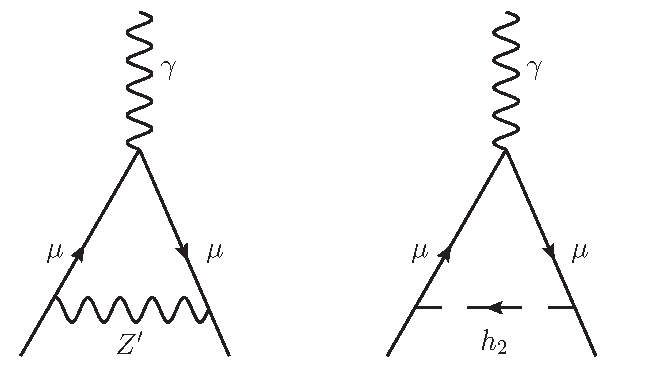
\includegraphics[scale=0.75]{/BLSM/g-2.pdf}
	\caption{One-loop diagrams contributing to $\Delta a_\mu^{\ro{NP}}$ in the B-L-SM.}
	\label{fig:g-2}
\end{figure}	
%%%%%%%%%%%%%%%%%%%%%%%%%

\subsection{Numerical discussion}

For the B-L-SM scan our scanning routine randomly samples parameter space points according to the ranges in Tab.~\ref{tab:scan}.
%
\begin{table}[H]
	\begin{center}
%\begin{ruledtabular}
		\begin{tabular}{ccccc}
			\toprule                     
			$\lambda_{1}$ & $\lambda_{2,3}$ & $g_{\mathrm{B-L}}$ & $g_{\mathrm{YB}}$ & $x~{\mathrm{[TeV]}}$  
			\\       
						\midrule 
			$\left[10^{-2},\; 10^{0.5}
			\right]$ 			    							& $\left[10^{-8},\; 10
			\right]$ 			    							& $\left[10^{-8},\; 10
			\right]$		& $\left[10^{-8},\; 10
			\right]$	&	$\left[0.5,\; 20.5
			\right]$ 	\\
			\bottomrule
		\end{tabular}  
		\caption{Parameter scan ranges used in our analysis. Note that the value of $\lambda_1$ is mostly constrained by the tree-level Higgs boson mass given in Eq.~\eqref{eq:simplify}. 
		}
		\label{tab:scan}
%\end{ruledtabular}
	\end{center}
\end{table}
%  
% { \color{gray} Keeping the remaining free parameters of the model to be in agreement with the Standard Model. } 
%
%The refereed checks applied were sequential and begin with the "zero-th" check where our spectrum generator \texttt{SPheno}, promptly rejects any scenario with tachyonic scalar masses and un-renormalizable quantities.  
%
%\texttt{SPheno} is a particle spectrum generator code written in Fortran 90. It's emphasis on easy generalisability and speed made it a natural part of our numerical analysis. It takes information about our models Lagrangian, such as fields, charges and fundamental symmetries, and creates a executable file capable of quickly generating a spectrum file with all details regarding mass, decay and flavour observables information in the standardized SUSY Les-Houches accord format. All generated spectrums are processed and stored. 
%
%This Lagrangian information is fed to \texttt{SPheno} also in standardized format automatically generated by a Mathematica packaged designed for such purposes called \texttt{SARAH}.  
%
%All inputs and outputs from \texttt{SPheno} are written in the format of a SUSY Les Houches Accord (SLHA) \cite{Skands:2003cj}. 
%
%All points that complete a "zero-th" layer, have all their information regarding two and three body decays, in particular to the Higgs bosons, passed along to another set Fortran 90 packages called \texttt{HiggsBounds} and \texttt{HiggsSignals}. These test experimental detection limits for the new scalars and verify if we have a "SM" like Higgs to account for the detected boson. 
% 
%After this is completed tabular files with all information collected from all programs is saved for later use.
%
%The presence of new bosons in the theory can lead to large deviations in EW precision observables. 

\subsubsection{Electroweak precision observables}

Typically, the most stringent constraints of the scalar sector emerge from the oblique $S,T,U$ parameters, which are also calculated by \texttt{SPheno}. 
%
This conecept was first introduced by Peskin and T. Takeuchi in Ref\,\cite{Peskin1992}.
%
Current precision measurements provide the allowed regions,
%
\begin{equation}
	S = 0.02 \pm 0.10\,, \qquad T = 0.07 \pm 0.12\,, \qquad U = 0.00 \pm 0.09
	\label{eq:oblique}
\end{equation}

%
where $S$-$T$ are $92\%$ correlated, while $S$-$U$ and $T$-$U$ are $-66\%$ and $-86\%$ anti-correlated, respectively.
%
We compare our results with the EW fit in Eq.~\eqref{eq:oblique} and require consistency with the best fit point within a $95\%$ C.L.~ellipsoid (see Ref.~\cite{Costa:2014qga} for further details about this method). %
%
In short we require that the contributions coming from new physics respect the EW precision tests within a 95\% C.L. ellipsoid by imposing, 
%
\begin{equation}
\Delta \chi \equiv \sum_{ij}  \left(  \Delta \mathcal{O}_{i}^{NP} - \mathcal{O}_{i}^{(0)} \right) [ ( \sigma^2 )^{-1} ]_{ij}  \left(  \mathcal{O}_{j}^{NP} - \mathcal{O}_{j}^{(0)}  \right) < 7.815    
\end{equation}
%
Where $\Delta \mathcal{O}_i^{NP} \equiv \mathcal{O}_i - \mathcal{O}^{SM} \rightarrow (\Delta S , \Delta T , \Delta U )$ being that, $\mathcal{O}_i^{(0)}$ is the deviation generated by the Higgs doulbet in the SM if his mass is 125.09. And where the covariance matrix expressed in terms of correlation matrix and started deviations can be seen in, 
\begin{equation}
[ \sigma^2 ]^{-1} \equiv \begin{pmatrix}
867.49 & −904.30 & -360.66\\
−904.30 & 1154.65 & 584.55 \\
−360.66 & 584.55 &  455.19
\end{pmatrix}  
\end{equation}
These values are seen in Ref\,\cite{Baak_2012}. 

We show in Fig.~\ref{fig:STU} our results in the $ST$ (left) and $TU$ (right) planes where black points are consistent with EW precision observables at $95\%$ C.L.~whereas grey ones lie outside the corresponding ellipsoid of the best fit point and, thus, the first points to be excluded in our analysis. 
%%%%%%%%%%%%%%%%%%%%%%%%%
\begin{figure}[H]
	\centering
	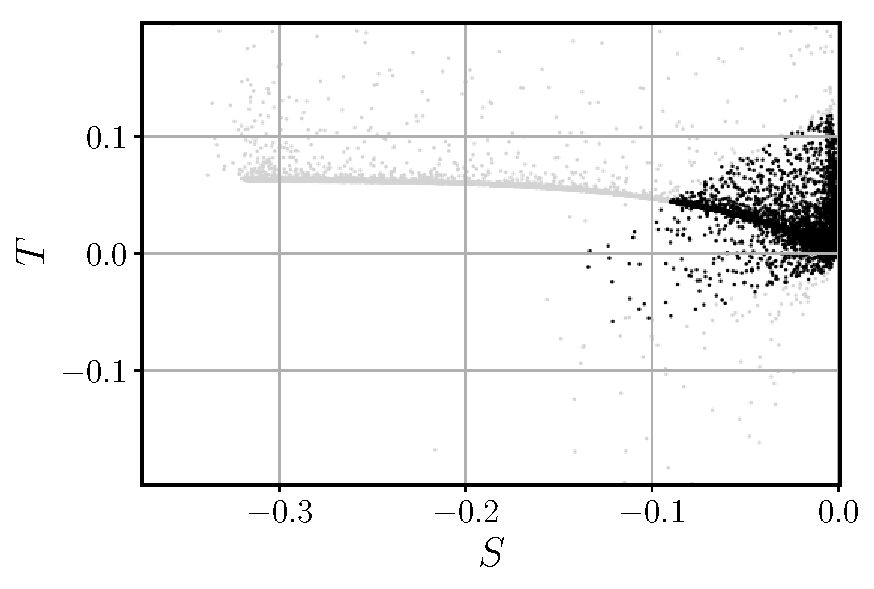
\includegraphics[scale=0.45]{/BLSM/ST.pdf}
	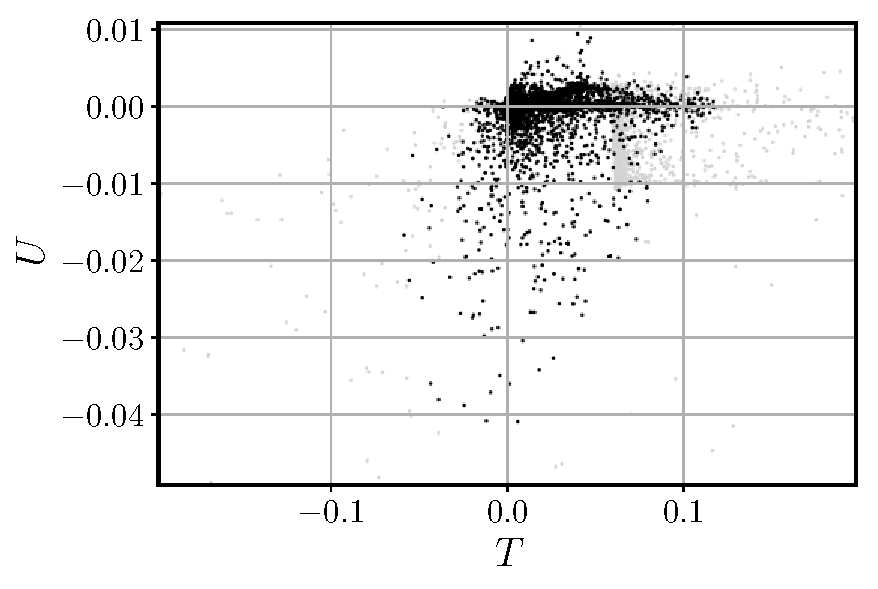
\includegraphics[scale=0.45]{/BLSM/TU.pdf}
	\caption{Scatter plots for EW precision observables showing the $ST$ (left) and $TU$ (right) planes. Accepted points lying within a $95\%$ C.L.~ellipsoid of the best fit point are represented in black whereas grey points are excluded.}
	\label{fig:STU}
\end{figure}	
%%%%%%%%%%%%%%%%%%%%%%%%%

%The B-L-SM predicts a new visible scalar, which we denote as $h_2$, in addition to a SM-like $125~\ro{GeV}$ Higgs boson, $h_1$. 

\subsubsection{Higgs Constraints}

As stated before, we confront the surviving scenarios, black points in Fig.~\ref{fig:STU}, with collider bounds. 
%
In particular the $95\%$ Confidance Level (C.L.) exclusion limits on a new scalar particle and check for consistency with the observed Higgs boson at $3 \sigma$. 
%
These Bounds are checked by \texttt{HiggsBounds/HiggsSignals},  which  is are a set of packages that test the theoretical predictions of our Model from against the exclusion bounds that have been set from Higgs searches at the LHC, LEP and the Tevatron. 
%
We have accepted points whose fit to the data replicates the observed signal at $95\%$ C.L.~while the measured value for its mass, $m_{h_1} = 125.10 \pm 0.14~\textrm{GeV}$ \cite{Tanabashi:2018oca}. 
%
The information required for this check is the the number of neutral and charged Higgs bosons and the information generated by the \texttt{SPheno} output in the format of a SUSY Les Houches Accord (SLHA) \cite{Skands:2003cj} file.
%
Specifically, \texttt{SPheno} provides scalar masses, total decay widths, Higgs decay branching ratios as well as the SM-normalized effective Higgs couplings to fermions and bosons squared (that are needed for analysis of the Higgs boson production cross sections). 
%
For details about this calculation, see Ref.~\cite{Bechtle:2013wla}.

The basic value calculated by \texttt{HiggsSignals} is the signal strength modifier $\mu_{x}$ which parametrizes the signal rate of a particular final state $x$ normalized to the SM expectation trougha a peak-centered $\chi^2$ statistical method.

The combined implementation of \texttt{HiggsBounds/HiggsSignals}, looks at the properties of the discovered Higgs and searches for additional Higgs states, which are then either excluded or allowed in the particle spectra of our model. 

%A  sister  computer  code  ofHiggsBoundsisHiggsSignals,  which  can  be  easily  im-plemented  in  the  exclusion  of  parameter  points.   The  computer  codeHiggsSignalsis,therefore,  a  natural  extension  ofHiggsBoundssince  both  take  as  input  the  number  ofneutral Higgs bosons, scalar masses, cross sections, branching ratios, among other physicalquantities.   The  basic  experimental  value  thatHiggsSignalsuses  is  thesignal  strengthmodifierμxx, which parametrizes the signal rate of a particular final statexx, normalizedto the SM expectation.  Finally,HiggsSignalsimplements the peak-centeredχ2method11There could be a compensation coming from the values of the VEVs.36
%to determine quantitatively to what degree the data and the predicted theory of the modelare compatible.  The combined implementation ofHiggsBounds/HiggsSignalslooks atthe properties of the discovered Higgs and searches for additional Higgs states, which arethen either excluded or allowed in the particle spectra of our model.  In our implementationof the 3HDM, we have found that all the points that passHiggsBoundsare extremely likelyto passHiggsSignalsas well due to the alignment limit imp

%For the latter, we have accepted points whose fit to the data replicates the observed signal at $95\%$ C.L.~while the measured value for its mass, $m_{h_1} = 125.10 \pm 0.14~\textrm{GeV}$ \cite{Tanabashi:2018oca}, is reproduced within a $3\sigma$ uncertainty. 
%The required input data for \texttt{HiggsBounds/HiggsSignals} are generated by the \texttt{SPheno} output in the format of a SUSY Les Houches Accord (SLHA) \cite{Skands:2003cj} file.
%
%In particular, it provides scalar masses, total decay widths, Higgs decay branching ratios as well as the SM-normalized effective Higgs couplings to fermions and bosons squared (that are needed for analysis of the Higgs boson production cross sections). For details about this calculation, see Ref.~\cite{Bechtle:2013wla}.
%
%On a third layer of phenomenological tests we have studied the viability of the surviving scenarios from the perspective of direct collider searches for a new $Z^\prime$ gauge boson. We have used \texttt{MadGraph5\_aMC@NLO 2.6.2} \cite{Alwall:2014hca} to compute the $Z^\prime$ Drell-Yan production cross section and subsequent decay into the first and second-generation leptons, i.e.~$ \sigma \left( pp \to Z^\prime \right) \times B \left( Z^\prime \to \ell \ell\right)$ with $\ell = e,\; \mu$, and then compared our results to the most recent ATLAS exclusion bounds from the LHC runs at the center-of-mass energy $\sqrt{s} = 13~\textrm{TeV}$ \cite{Aaboud:2017buh}. The \texttt{SPheno} SLHA output files were used as parameter cards for \texttt{MadGraph5\_aMC@NLO}, where the information required to calculate $ \sigma\left(pp \to Z^\prime\right) \times B\left(Z^\prime \to \ell \ell\right()$, such as the $Z^\prime$ boson mass, its total width and decay branching ratios into lepton pairs, is provided. 
%
\subsubsection{$Z^\prime$ Constraints}

From here we move onto the third layer of phenomenological tests we look at the viability of the surviving points from the perspective of direct collider searches for a new $Z^\prime$ gauge boson at the most recent collider experiments.
%
We have used \texttt{MadGraph5\_aMC@NLO 2.6.2} \cite{Alwall:2014hca}, with it we compute the $Z^\prime$ Drell-Yan production cross section and subsequent decay into the first and second-generation leptons, i.e.~$ \sigma \left( pp \to Z^\prime \right) \times B \left( Z^\prime \to \ell \ell\right)$ with $\ell = e,\; \mu$, and then compared our results to the most recent ATLAS exclusion bounds from the LHC runs at the center-of-mass energy $\sqrt{s} = 13~\textrm{TeV}$ \cite{Aaboud:2017buh}.

The \texttt{SPheno} SLHA output files were used as parameter cards for \texttt{MadGraph5\_aMC@NLO}, where the information required to calculate $ \sigma\left(pp \to Z^\prime\right) \times B\left(Z^\prime \to \ell \ell\right()$, such as the $Z^\prime$ boson mass, its total width and decay branching ratios into lepton pairs, is provided. 
%
% In this article, we study whether the muon anomalous magnetic moment can be totally or partially explained in the model under consideration and all scenarios with an excessive contribution to $\Delta a_\mu^{\textrm{NP}}$ larger than the upper $2 \sigma$ bound in Eq.~(\ref{g-2}) were rejected.
%
%\subsubsection{Discussion of numerical results}
%\label{sec:discuss}
%
%
Let us now discuss the phenomenological properties of the B-L-SM model. First, we focus on the current collider constraints and study their impact on both the scalar and gauge sectors.
%%%%%%%%%%%%%%%%%%%%%%%%%
\begin{figure}[H]
	\centering
	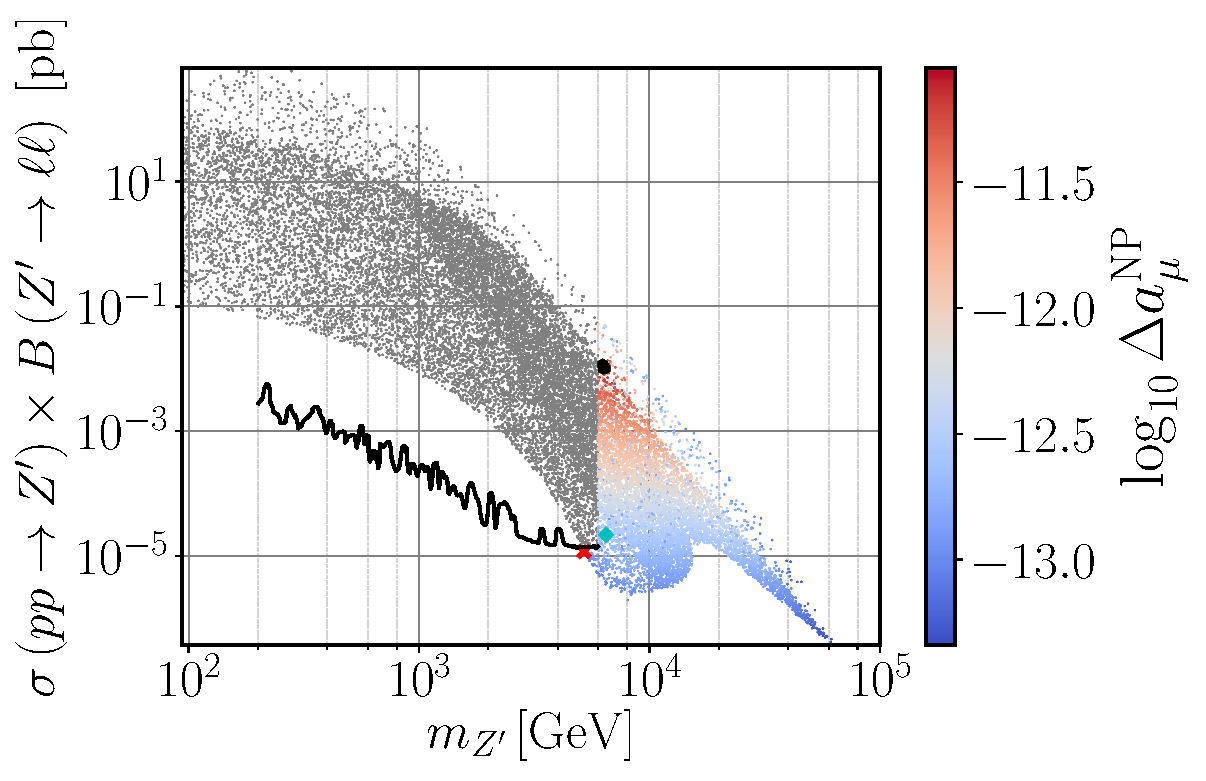
\includegraphics[scale=0.37]{/BLSM/mZp_Xsec_Amu.pdf}
	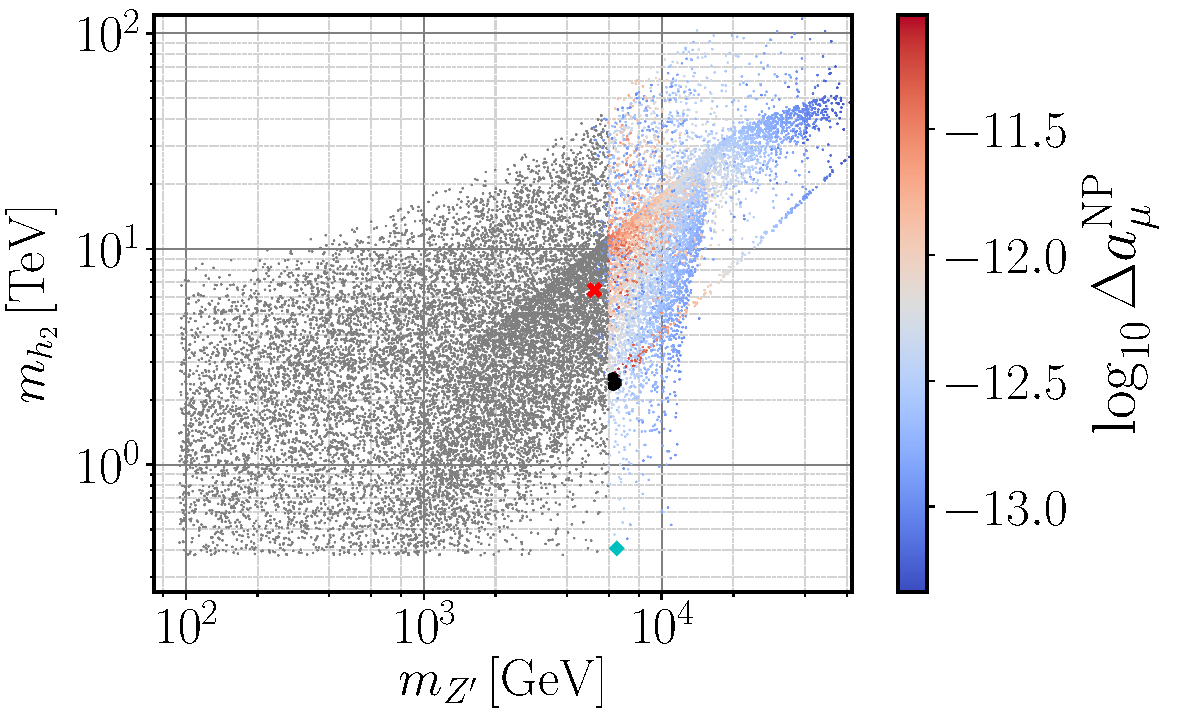
\includegraphics[scale=0.37]{/BLSM/mZp_Mhp_Amu.pdf}
	\caption{Scatter plots showing the $Z^\prime$ Drell-Yan production cross section times the decay branching ratio into a pair of electrons and muons (left panel) and the new scalar mass $m_{h_2}$ (right panel) as functions of $m_{Z^\prime}$ and the new physics (NP) contributions to the muon $\Delta a_\mu$ anomaly. Coloured points have survived all theoretical and experimental constraints while grey points are excluded by direct $Z^\prime$ searches at the LHC. The region between the two dashed lines represents the current ATLAS expected limit on the production cross section times branching ratio into a pair of leptons at $95\%$ C.L.~and is taken from the plot in Fig.~4 of Ref.~\cite{Aaboud:2017buh}. The four highlighted points in both panels denote the benchmark scenarios described in detail in Tab.~\ref{tab:bench}.}
	\label{fig:Plots1}
\end{figure}	
%%%%%%%%%%%%%%%%%%%%%%%%%

We show in Fig.~\ref{fig:Plots1} the scenarios generated in our parameter space scan (see Tab.~\ref{tab:scan}) that have passed all theoretical constraints such as boundedness from below, unitarity and EW precision tests, and experimental restrictions, such as the compatability with the SM Higgs data and where a new visible scalar $h_2$ is unconstrained by the direct collider searches.
%
On the left panel, we show the $Z^\prime$ production cross section times its branching ratio to the first- and second-generation leptons, $\sigma B \equiv \sigma \left( pp \to Z^\prime \right) \times B \left( Z^\prime \to \ell \ell \right) $ with $\ell = e,\mu$, as a function of the new vector boson mass and the new physics contribution to the muon anomalous magnetic moment $\Delta a^{\textrm{NP}}_\mu$ (colour scale). 
%
On the right panel, we show the new scalar mass as a function of the $Z^\prime$ Mass. 
%
All points above the red dashed line are excluded at $95\%$ C.L.~by the upper expected limit on $Z^\prime$ direct searches at the LHC by the ATLAS experiment and are represented in grey shades. 
%
Darker shades denote \textit{would-be-scenarios} with larger values of $\Delta a^{\textrm{NP}}_\mu$ while the smaller contributions to the muon $\left(g-2\right)_\mu / 2$ anomaly are represented with the lighter shades. 
%
The region between the two dashed lines corresponds to the $Z^\prime$ ATLAS limit with a $2\sigma$ uncertainty represented by the yellow band in Fig.~4 of \cite{Aaboud:2017buh}.
%
Provided that the observed limit by the ATLAS detector lies within this region we have taken a conservative approach and accepted all points whose $\sigma B$ value lies below the red dashed line (upper limit) in Fig.~\ref{fig:Plots1}.
%
The blue dashed line, which corresponds to the stricter $2 \sigma$ lower bound, is only shown for completeness of information. The red cross in our figures signals the lightest $Z^\prime$ found in our scan which we regard as a possible early-discovery (or early-exclusion) benchmark point in the forthcoming LHC runs. Such a benchmark point is shown in the first line of Tab.~\ref{tab:bench}.
%
On the right panel, we notice that the new scalar bosons can become as light as $380 - 400~\textrm{GeV}$, but with $Z^\prime$ masses in the range of $5 - 9~\textrm{TeV}$. We highlight with a magenta diamond the benchmark point with the lightest $Z^\prime$ boson within this range. 
%
This point is shown in the second line of Tab.~\ref{tab:bench}.
%
\begin{table}[H]
	\begin{center}
	%\resizebox{\columnwidth}{!}{%
%\begin{ruledtabular}
		\begin{tabular}{cccccccc}
			% \toprule                     
			$m_{Z^\prime}$ & $m_{h_2}$ &  $x$ & $ \log_{10} \Delta a_\mu^{\ro{NP}}$ & $\sigma B$ & $\theta_W^\prime$ & $\alpha_h$ & $g_{\ro{B-L}} \simeq g^{\ell \ell Z^\prime}$ \vspace{1mm}
			\\
			\hline \vspace{-2mm} \\ 
			%%%%%%%%%%
			$3.13$ 			    							& $3.72$ 			    				& $15.7$		& $-12.1$	&	$2.22\times 10^{-4}$ &	$\approx 0$ &	$5.67 \times 10^{-5}$ &	$0.0976$\vspace{1mm} 	\\
			%%%%%%%%%%
			$5.37$ 			    							& $0.396$ 			    				& $9.10$		& $-11.7$	&	$4.23 \times 10^{-5}$ &	$2.55 \times 10^{-7}$ &	$9.44 \times 10^{-7}$ &	$0.302$\vspace{1mm}  	\\
			%%%%%%%%%%
			$7.35$ 			    							& $1.49$ 			    				& $0.321$		& $-8.75$	&	$0.0115$ &	$1.83 \times 10^{-7}$ &	$1.20 \times 10^{-6}$ &	$3.15$\vspace{1mm}  	\\
			%%%%%%%%%%
			$5.91$ 			    							& $1.32$ 			    				& $0.335$		& $-8.78$	&	$0.0285$ &	$1.30 \times 10^{-4}$ &	$1.04 \times 10^{-5} $ &	$2.94$\vspace{1mm}  	\\
%			\bottomrule
		\end{tabular}
%		\end{ruledtabular}
		%}
		\caption{A selection of four benchmark points represented in Figs.~\ref{fig:Plots1}, \ref{fig:Plots4} to \ref{fig:Plots2}. The $m_{Z^\prime}$, $m_{h_2}$ and $x$ parameters are given in TeV. The first line represents a point with light $h_2$ while the second line shows the lightest allowed $Z^\prime$ boson found in our scan. The last two lines show two points that reproduce the observed value of the muon $(g-2)$ within $1\sigma$ uncertainty.}
		\label{tab:bench}
	\end{center}
\end{table}
% 
\subsubsection{Implications of direct $Z^\prime$ searches at the LHC for the $\left(g-2\right)_\mu$ anomaly}

Looking again to Fig.~\ref{fig:Plots1} (left panel), we see that there is a thin dark-red stripe where $\Delta a^{\ro{NP}}_\mu$ explains the observed anomaly shown in Eq.~(\ref{g-2}) for a range of $m_{Z^\prime}$ boson masses approximately between $5~\ro{TeV}$ and $20~\ro{TeV}$. This region is particularly interesting as it can be partially probed by the forthcoming LHC runs or at future colliders. If a $Z^\prime$ boson discovery remains elusive for such a mass range, it can exclude a possibility of explaining the muon $\left(g-2\right)_\mu$ anomaly in the context of the B-L-SM. It is also worth noticing that such preferred $\Delta a^{\ro{NP}}_\mu$ values represent a small island in the right plot of Fig.~\ref{fig:Plots1} where the new scalar boson mass is restricted to the range of $1~\ro{TeV} < m_{h_2} < 4~\ro{TeV}$.


Since the couplings of a new scalar $h_2$ to the SM fermions are suppressed by a factor of $\sin \alpha_h$, which we find to be always smaller than $0.08$ as can be seen in the bottom panel of Fig.~\ref{fig:Plots4}, the right diagram in Fig.~\ref{fig:g-2}, which scales as $\Delta a_\mu^{h_2} \propto {m_\mu^2}/{m_{h_2}^2}\left(y_\mu \sin \alpha_h\right)^2$ with $\sin^2 \alpha_h < 0.0064$ and $y_\mu = Y_e^{22}$, providing sub-leading contributions to $\Delta a_{\mu}$. Furthermore, as we show in the top-left panel of Fig.~\ref{fig:Plots4} the new scalar boson mass, which we have found to satisfy $m_{h_2} \gtrsim 380~\ro{GeV}$, is not light enough to compensate the smallness of the scalar mixing angle. Conversely,  the new $Z^\prime$ boson can have sizeable couplings to fermions via gauge interactions proportional to $g_{\rm B-L}$. Therefore, the left diagram in Fig.~\ref{fig:g-2} provides the leading contribution to the $\left(g-2\right)_\mu$ in the model under consideration.
%%%%%%%%%%%%%%%%%%%%%%%%%
\begin{figure}[!htb]
	\centering
	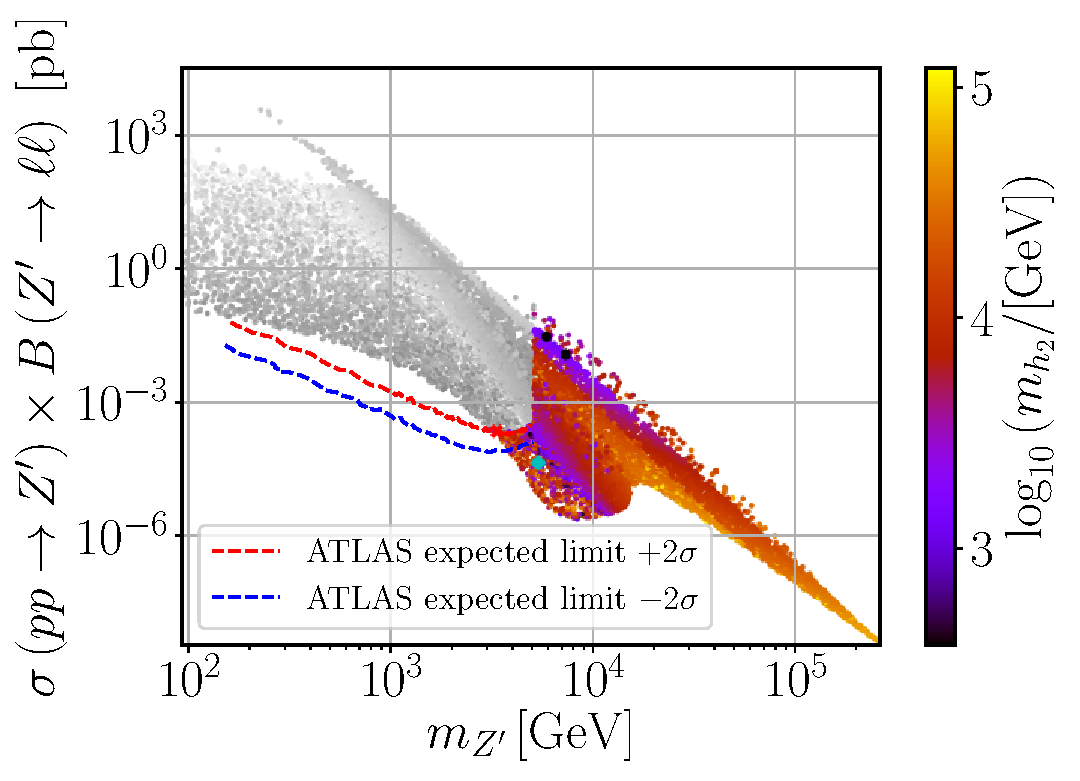
\includegraphics[scale=0.37]{/BLSM/mZp_Xsec_mh2.pdf}
	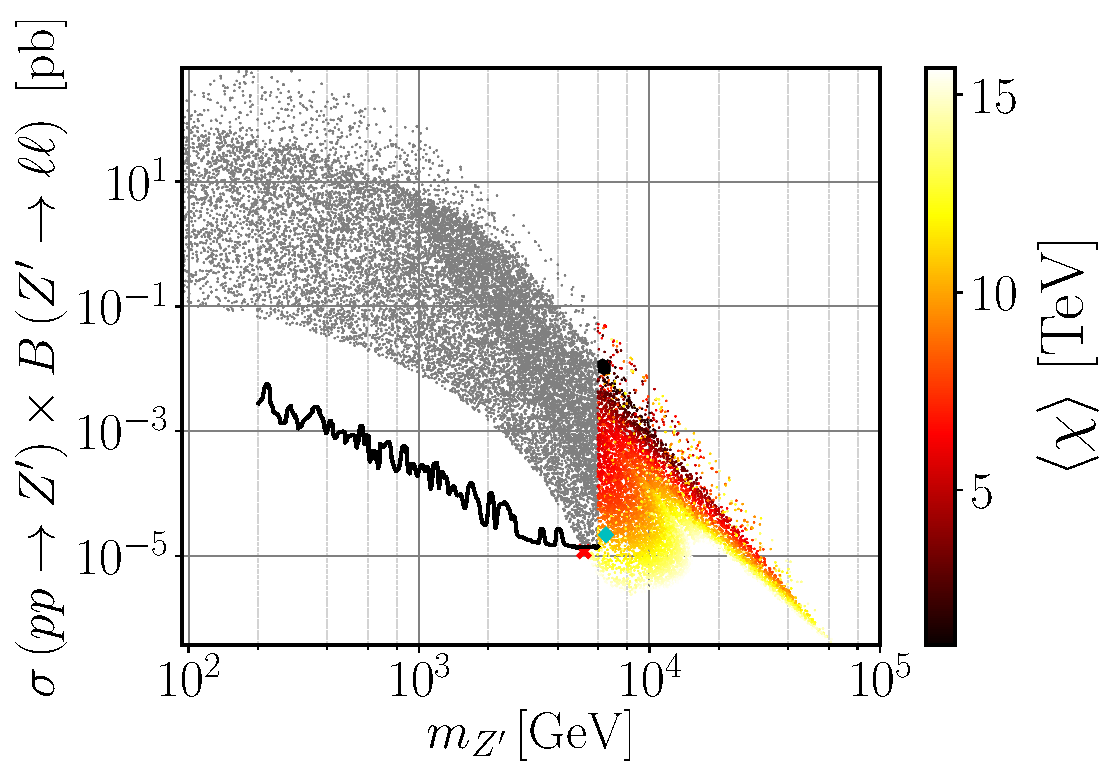
\includegraphics[scale=0.37]{/BLSM/mZp_Xsec_VEV.pdf}
	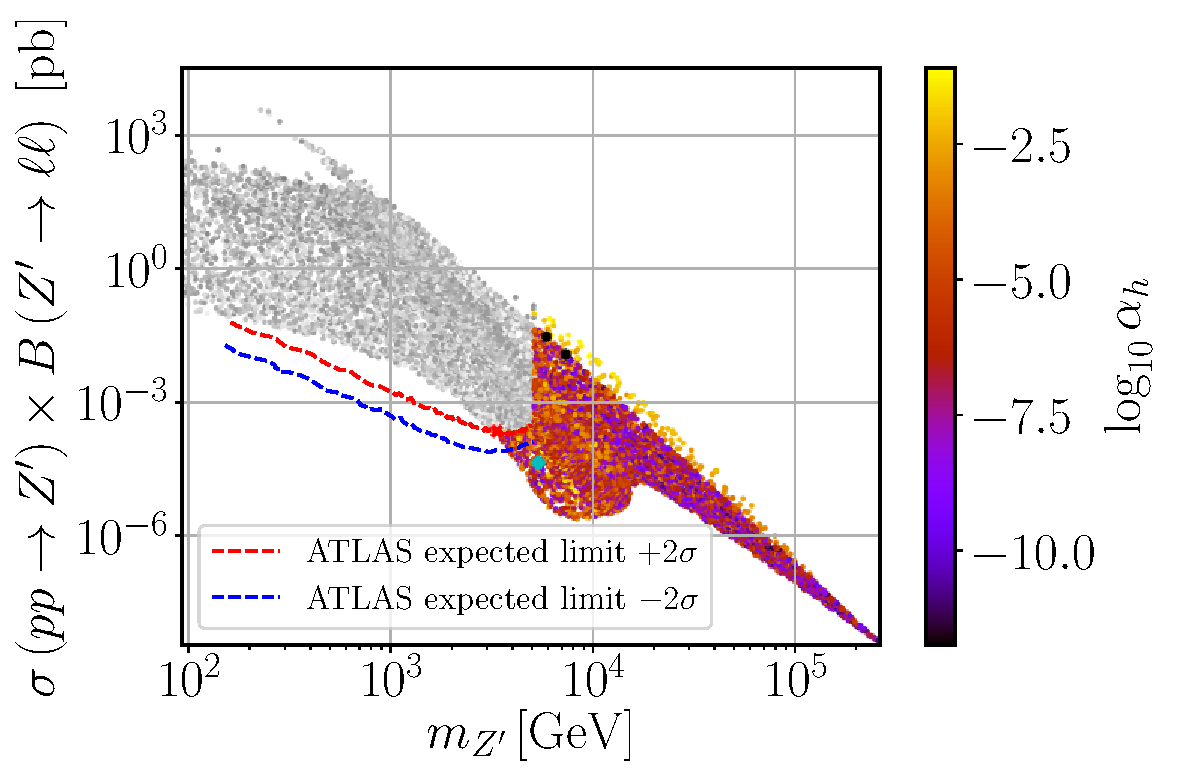
\includegraphics[scale=0.37]{/BLSM/mZp_Xsec_alpha.pdf}	
	\caption{Scatter plots showing the $Z^\prime$ Drell-Yan production cross section times the decay branching ratio into a pair of electrons and muons in terms of the $m_{Z^\prime}$ boson mass. The colour gradation represents the new scalar mass (top-left), the ratio between the EW- and $\U{B-L}$-breaking VEVs (top-right) and the scalar mixing angle (bottom). The grey points are excluded by direct $Z^\prime$ searches at the LHC. The four benchmark points in Tab.~\ref{tab:bench} are represented by the black dots (last two rows), cyan diamond (first row) and red cross (second row).}
	\label{fig:Plots4}
\end{figure}	
%%%%%%%%%%%%%%%%%%%%%%%%%
In particular, $\Delta a_\mu^{Z^\prime}$ is given by \cite{Freitas:2014pua}
\begin{equation}
\Delta a_\mu^{Z^\prime} = \tfrac{1}{12 \pi^2} \tfrac{m_{\mu}^2}{m_{Z^\prime}^2} \(3 g_{\rm L}^{\mu \mu Z^\prime} g_{\rm R}^{\mu \mu Z^\prime} - {g_{\rm L}^{\mu \mu Z^\prime}}^2 - {g_{\rm R}^{\mu \mu Z^\prime}}^2 \)
\label{eq:ZpContribution}
\end{equation}
where the left- and right-chiral projections of the charged lepton couplings to the $Z^\prime$ boson, $g_{\rm L}^{\ell \ell Z^\prime}$ and $g_{\rm R}^{\ell \ell Z^\prime}$, respectively, can be approximated as follows
\begin{equation}
\begin{aligned}
    g_{\rm L}^{\ell \ell Z^\prime} &\simeq g_{\rm B-L} + \tfrac{1}{32} \(\tfrac{v}{x}\)^2 \tfrac{g_{\rm YB}}{g_{\rm B-L}} \[g_{\rm Y}^2 - g^2 + 2 g_{\rm Y}g_{\rm YB}\]\,,
    \\
    g_{\rm R}^{\ell \ell Z^\prime} &\simeq g_{\rm B-L} + \tfrac{1}{16} \(\tfrac{v}{x}\)^2 \tfrac{g_{\rm YB}}{g_{\rm B-L}} \[g_{\rm Y}^2 + g_{\rm Y}g_{\rm YB}\]\,,
\end{aligned}\label{eq:gllZ}
\end{equation}
to second order in $v/x$-expansion. If $v/x \ll 1$, corresponding to the darker shades of the color scale in the top-right panel of Fig.~\ref{fig:Plots4}, we can further approximate
%
\begin{equation}
    g_{\rm L}^{\ell \ell Z^\prime} \simeq g_{\rm R}^{\ell \ell Z^\prime} \simeq g_{\ro{B-L}}\,,
    \label{eq:gLgR-simp}
\end{equation}
%
such that the muon anomalous magnetic moment gets significantly simplified to
\begin{equation}
\Delta a_\mu^{Z^\prime} \simeq \dfrac{g_{\ro{B-L}}^2}{12 \pi^2} \dfrac{m_{\mu}^2}{m_{Z^\prime}^2}\,.
\label{eq:amu-simple}
\end{equation}
%
Similarly, for the yellow band in the bottom of Fig.~\ref{fig:Plots3}, which corresponds to the region where $\Delta a_{\mu}^{\rm NP}$ is maximized (see top-left panel of Fig.~\ref{fig:Plots1}), a large value of the $\U{B-L}$ gauge coupling also allows one to simplify Eq.~\eqref{eq:ZpContribution} reducing it to the form of Eq.~\eqref{eq:amu-simple}. This is in fact what we have observed and, for the yellow band region, we see in the bottom panel of Fig.~\ref{fig:Plots3} that $g_{\ro{B-L}} \simeq 3$. A sizeable value of $g_{\ro{B-L}}$ is indeed what is contributing to the enhancement of $\Delta a_{\mu}^{\rm NP}$, in particular, for the red region in both panels of Fig.~\ref{fig:Plots1}. We show in the third and fourth lines of Tab.~\ref{tab:bench} the two benchmark points that better reproduce the muon anomalous magnetic moment represented by two black dots in
Figs.~\ref{fig:Plots1}, \ref{fig:Plots4} to \ref{fig:Plots2}.
%%%%%%%%%%%%%%%%%%%%%%%%%
\begin{figure}[!htb]
	\centering
	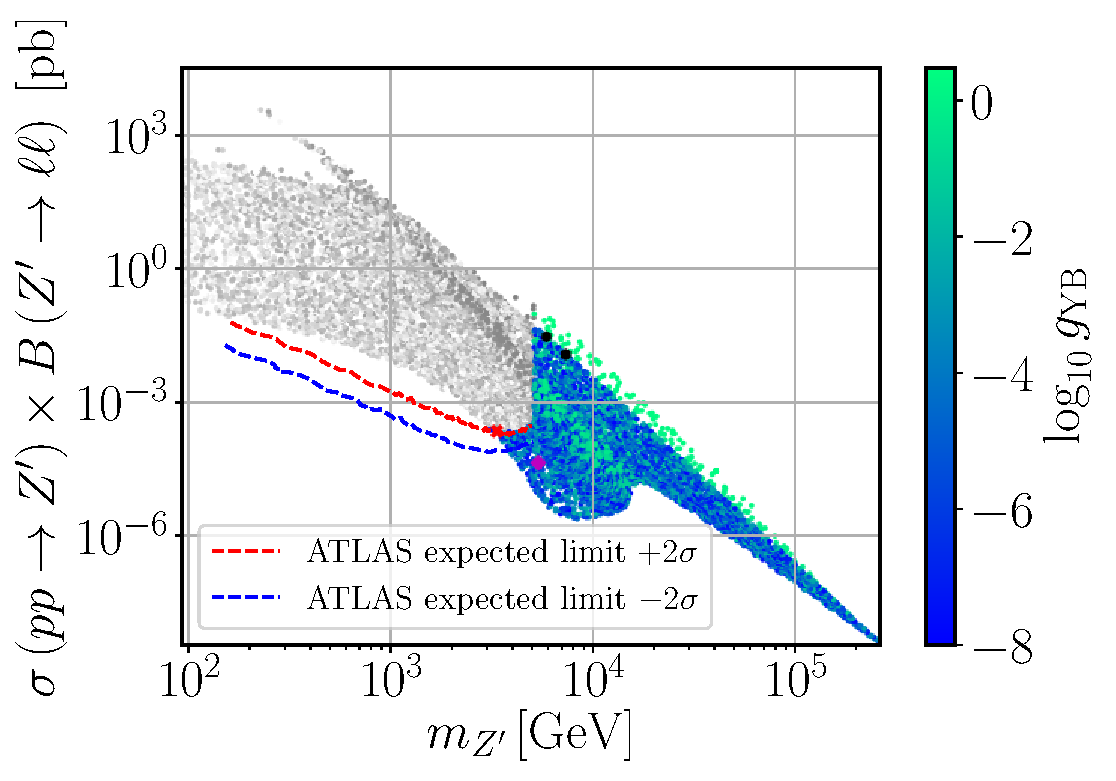
\includegraphics[scale=0.37]{/BLSM/mZp_Xsec_gYB.pdf}
	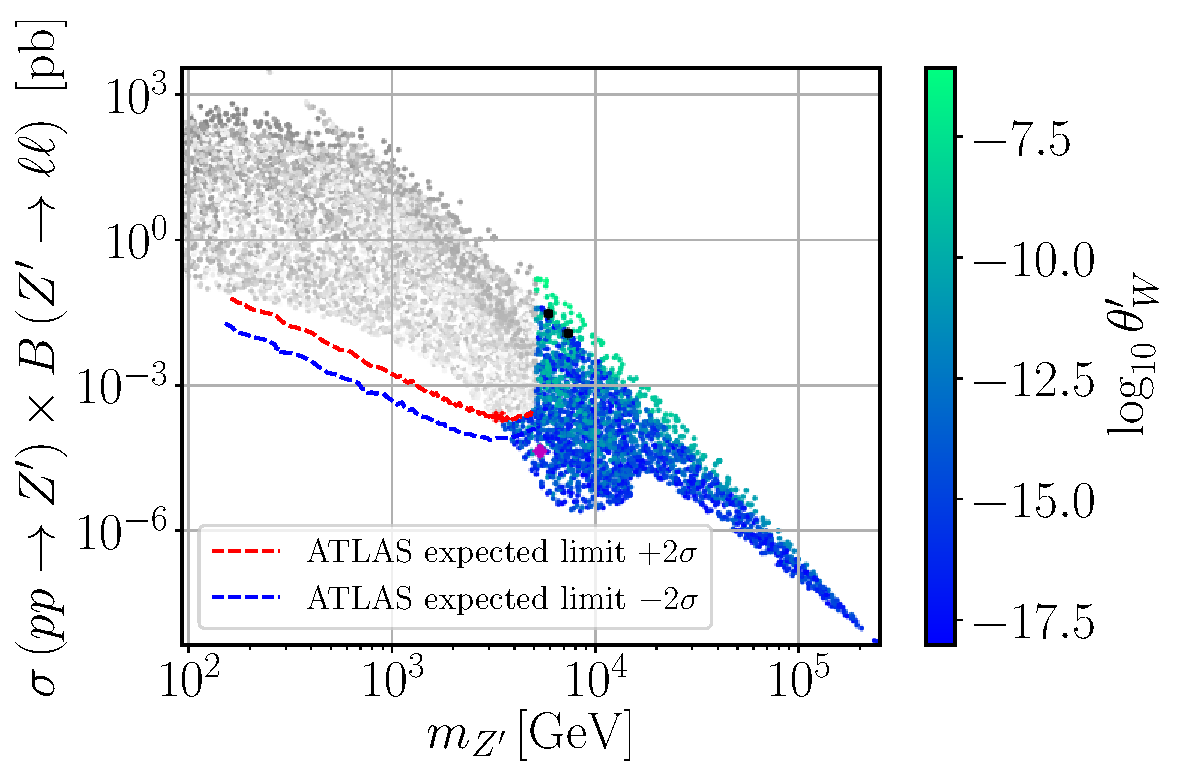
\includegraphics[scale=0.37]{/BLSM/mZp_Xsec_twp.pdf}
	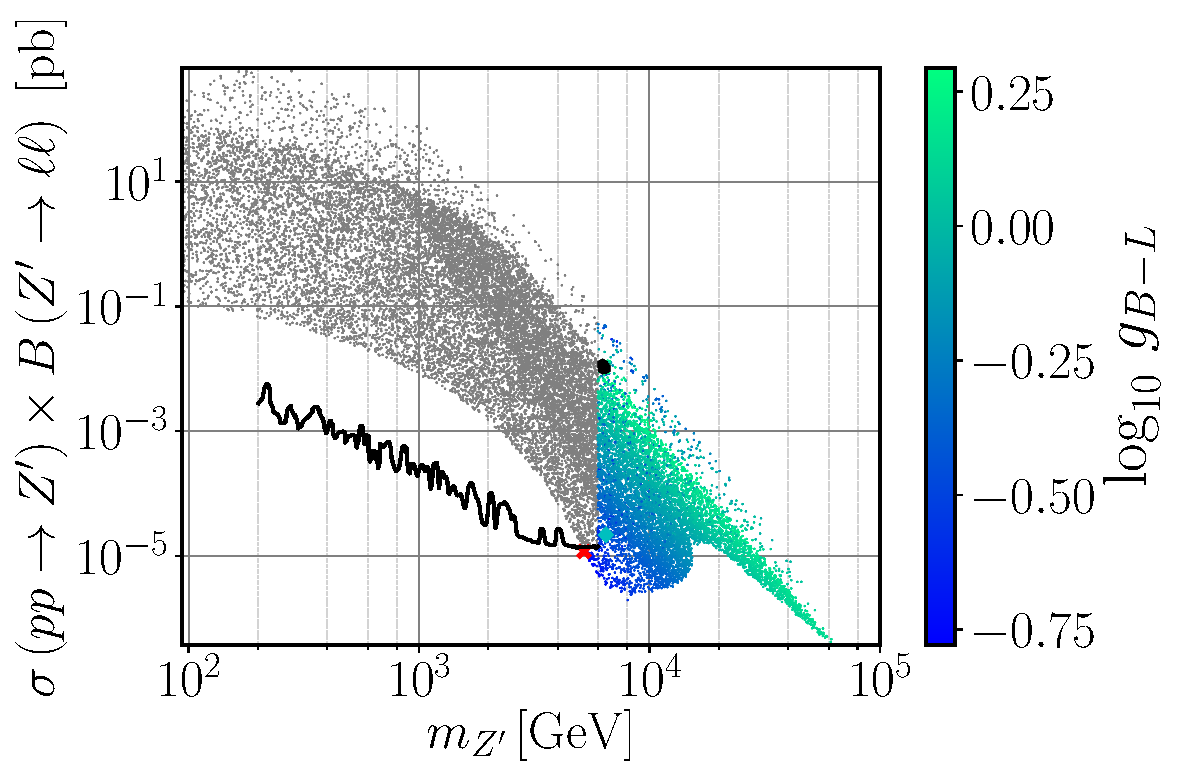
\includegraphics[scale=0.37]{/BLSM/mZp_Xsec_gBL.pdf}	
	\caption{The same as in Fig.~\ref{fig:Plots4} but with the colour scale representing the gauge-mixing parameters $g_{\ro{YB}}$ (top-left), $\theta_{W}^{\prime}$ (top-right), and the $\U{B-L}$ gauge coupling (bottom).}
	\label{fig:Plots3}
\end{figure}	
%%%%%%%%%%%%%%%%%%%%%%%%%

In fact, a close inspection of Fig.~\ref{fig:Plots1} (left panel) and Fig.~\ref{fig:Plots4} (top-right panel) reveals an almost one-to-one correspondence between the colour shades. 
This suggests that $\Delta a_{\mu}^{Z^\prime}$ must somehow be related to the VEV ratio $v/x$. 
To understand this behaviour, let us also look to Fig.~\ref{fig:Plots3} (top-left panel) where we see that the kinetic-mixing gauge coupling $g_{\ro{YB}}$ is typically very small apart from two green bands where it can become of order $\mathcal{O}(1)$.
Interestingly, whenever $g_{\ro{YB}}$ becomes sizeable, $v/x \ll 1$ is realised, which means that Eq.~\eqref{eq:mZ} is indeed a good approximation as was argued above. It is then possible to eliminate $g_{\ro{B-L}}$ from Eq.~\eqref{eq:amu-simple} and rewrite it as
\begin{equation}
    \Delta a_\mu^{Z^\prime} \simeq \dfrac{y_\mu^2}{96 \pi^2} \(\dfrac{v}{x}\)^2 \,,
    \label{eq:amu-vev}
\end{equation}
which explains the observed correlation between both Fig.~\ref{fig:Plots1} (left panel) and Fig.~\ref{fig:Plots4} (top-right panel) and, for instance, the thin red stripe of points is compatible with a full description of the muon $\left(g-2\right)_{\mu}/2$ anomaly. Note that this simple and illuminating relation becomes valid as a consequence of the heavy $Z^\prime$ mass regime, in combination with the smallness of the $\theta_{W}^{\prime}$ mixing angle required by LEP constraints. Indeed, while we have not imposed any strong restriction on the input parameters of our scan (see Tab.~\ref{tab:scan}), Eq.~\eqref{eq:theta-p} necessarily implies that both $g_{\ro{YB}}$ and $v/x$ cannot be simultaneously sizeable in agreement with what is seen in Fig.~\ref{fig:Plots3} (top-left panel) and Fig.~\ref{fig:Plots4} (top-right panel). The values of $\theta_W^\prime$ obtained in our scan are shown in the top-right panel of Fig.~\ref{fig:Plots3}.

For completeness, we show in Fig.~\ref{fig:Plots2} the physical couplings of $Z^\prime$ to muons (top panels) and to $W^\pm$ bosons (bottom panel).
%%%%%%%%%%%%%%%%%%%%%%%%%
\begin{figure}[!htb]
	\centering
	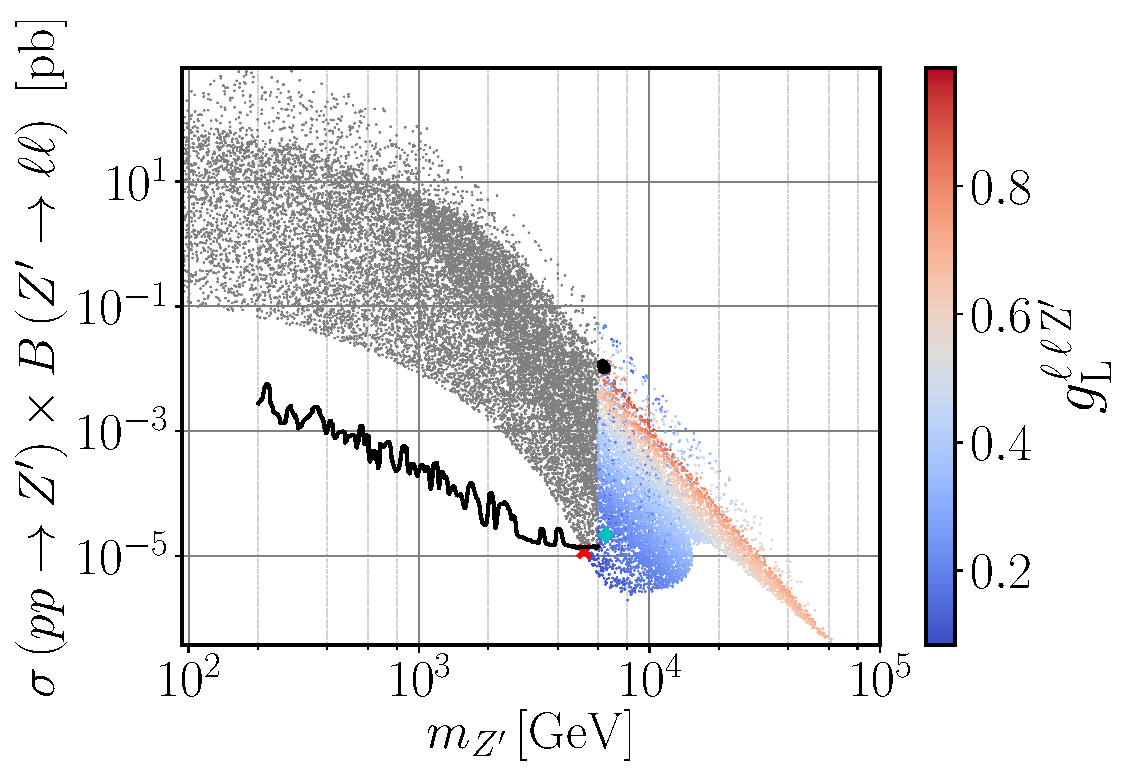
\includegraphics[scale=0.37]{/BLSM/mZp_Xsec_gLmumuZ.pdf}
	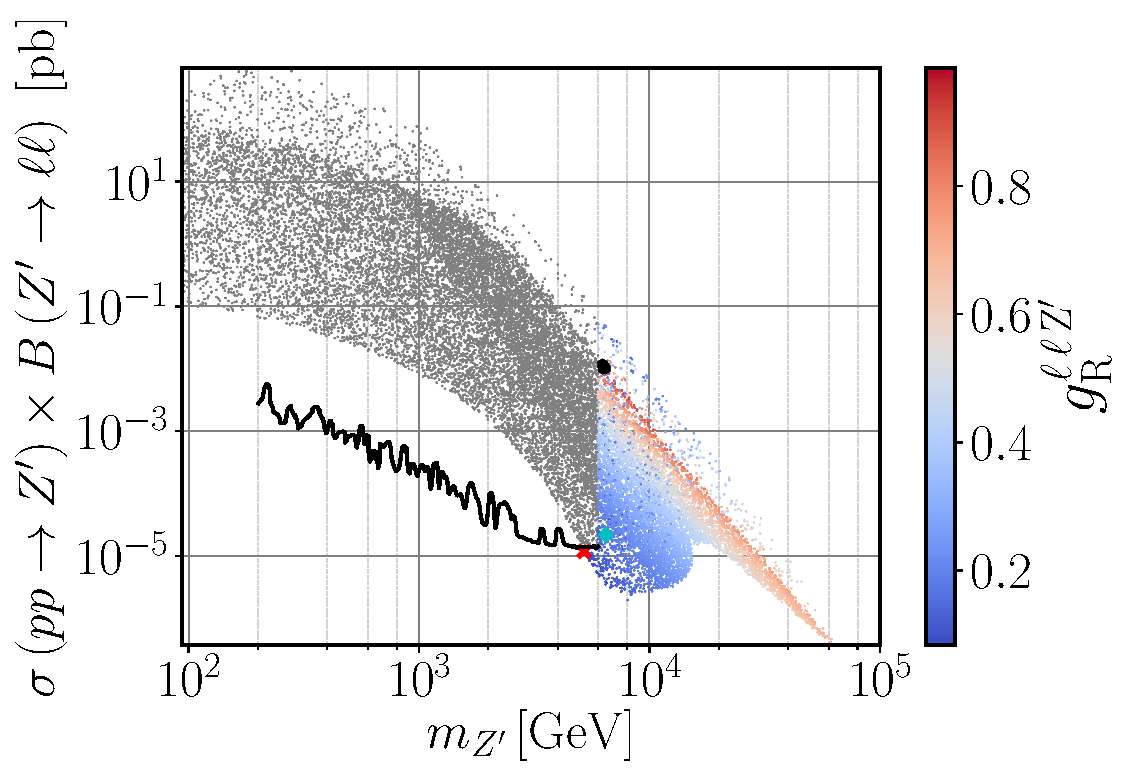
\includegraphics[scale=0.37]{/BLSM/mZp_Xsec_gRmumuZ.pdf}
	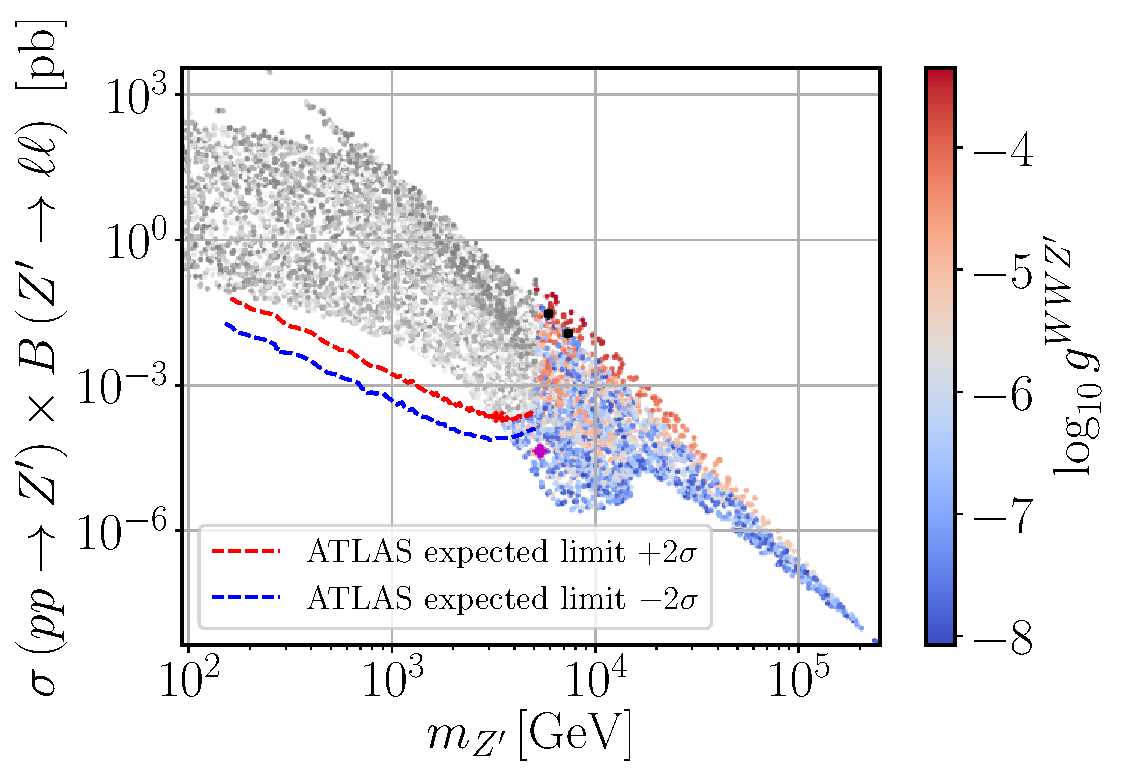
\includegraphics[scale=0.37]{/BLSM/mZp_Xsec_gWWZp.pdf}
	\caption{The same as in Fig.~\ref{fig:Plots4} but with the colour scale representing the coupling of leptons to the $Z^\prime$ (top panels) and the coupling of $W$ bosons to $Z^\prime$.}
	\label{fig:Plots2}
\end{figure}	
%%%%%%%%%%%%%%%%%%%%%%%%%
Note that, for the considered scenarios, the latter can be written as
\begin{equation}
    g^{WWZ^\prime} \simeq \dfrac{1}{16} \dfrac{g_{\ro{YB}}}{g_{\ro{B-L}}} \(\dfrac{v}{x}\)^2\,.
    \label{eq:gWWZp}
\end{equation}
While both $g_{\ro{B-L}}$ and the ratio $v/x$ provide a smooth continuous contribution in the $\sigma B - m_{Z^\prime}$ projection of the parameter space, the observed blurry region in $g^{WWZ^\prime}$ is correlated with the one in the top-left panel of Fig.~\ref{fig:Plots3} as expected from Eq.~\eqref{eq:gWWZp}. On the other hand, the couplings to leptons $g_{\rm L,R}^{\ell \ell Z^\prime}$ exhibit a strong correlation with $g_{\ro{B-L}}$ in Fig.~\ref{fig:Plots3}, in agreement with our discussion above and with Eq.~\eqref{eq:gLgR-simp}.

\subsubsection{Barr-Zee type contributions}
\label{sec:BarrZee}

To conclude our analysis, one should note that the two-loop Barr-Zee type diagrams \cite{Barr:1990vd} are always sub-dominant in our case. To see this, let us consider the four diagrams shown in Fig.~\ref{fig:Barr-Zee}.
%%%%%%%%%%%%%%%%%%%%%%%%%
\begin{figure}[!htb]
	\centering
	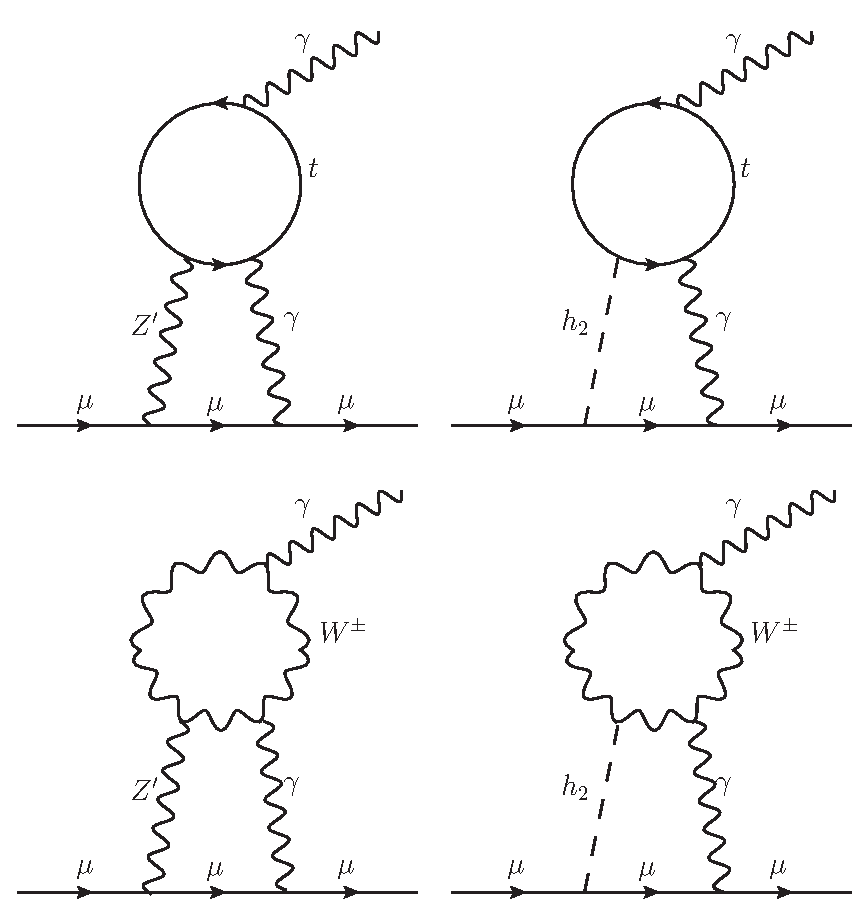
\includegraphics[scale=0.6]{/BLSM/Barr-Zee.pdf}
	\caption{Barr-Zee type two-loop diagrams contributing to $\Delta a_\mu$.}
	\label{fig:Barr-Zee}
\end{figure}	
%%%%%%%%%%%%%%%%%%%%%%%%%
The same reason that suppresses the one-loop $h_2$ contribution in Fig.~\ref{fig:g-2} is also responsible for the suppression of both the top-right and bottom-right diagrams in Fig.~\ref{fig:Barr-Zee} (for details see e.g.~Ref.~\cite{Ilisie:2015tra}). Recall that the coupling of $h_2$ to the SM particles is proportional to the scalar mixing angle $\alpha_h$, which is always small (or very small) as we can see in Fig.~\ref{fig:Plots4}. An analogous effect is present in the diagram involving a $W$-loop, where a vertex proportional to $g^{WWZ^\prime}$ suppresses such a contribution. The only diagram that might play a sizeable role is the top-left one where the couplings of $Z^\prime$ to both muons and top quarks are not negligible.

Let us then estimate the size of the first diagram in Fig.~\ref{fig:Barr-Zee}. This type of diagrams were already calculated in Ref.~\cite{Feng:2009gn} but for the case of a SM $Z$-boson. Since the same topology holds for the considered case of B-L-SM too, 
if we trade $Z$ by the new $Z^\prime$ boson, the contribution to the muon $(g-2)_\mu$ anomaly can be rewritten as
\begin{equation}
    \Delta a_{\mu}^{\gamma Z^\prime} = -\dfrac{g^2 g^2_{\ro{B-L}} m_\mu^2 \tan^2{\theta_W}}{1536 \pi^4} \left( g_{\ro{L}}^{ttZ^\prime} - g_{\ro{R}}^{ttZ^\prime} \right) \ro{T}_7\left( m_{Z^\prime}^2, m_t^2, m_t^2 \right)\,,
    \label{eq:agZ}
\end{equation}
where $T_7$ is a loop integral described in appendix \ref{app:T7}. The parameters $g_{\ro{L,R}}^{ttZ^\prime}$, calculated in \texttt{SARAH}, are the left- and right-chirality projections of the $Z^\prime$ coupling to top-quarks, given by
\begin{equation}
\begin{aligned}
    g_{\ro{L}}^{ttZ^\prime} &= -\dfrac{g_{\ro{B-L}}}{3} \cos{\theta_W^\prime} + \dfrac{g}{2} \cos{\theta_W} \sin{\theta_W^\prime} - \dfrac{g_{\ro{Y}}}{6} \sin{\theta_W} \sin{\theta_W^\prime} - \dfrac{g_{\ro{YB}}}{3} \sin{\theta_W} \sin{\theta_W^\prime}\,,
    \\
    g_{\ro{R}}^{ttZ^\prime} &= -\dfrac{g_{\ro{B-L}}}{3} \cos{\theta_W^\prime} - \dfrac{2 g_{\ro{Y}}}{3} \sin{\theta_W} \sin{\theta_W^\prime} - \dfrac{g_{\ro{YB}}}{3} \sin{\theta_W} \sin{\theta_W^\prime}\,.
\end{aligned}
\end{equation}
The loop integral $\ro{T}_7 \(m_{Z^\prime}^2, m_t^2, m_t^2\)$ was determined in Ref.~\cite{Feng:2009gn} and, in the limit $m_{Z^\prime} \gg m_t$, as we show in Eq.~\eqref{eq:T7-expanded}, it gets simplified to
\begin{equation}
    \ro{T}_7 \(m_{Z^\prime}^2, m_t^2, m_t^2\) \simeq \frac{2}{m_{Z^\prime}^2} \,,
    \label{eq:T7}
\end{equation}
up to a small truncation error (see Appendix~\ref{app:T7} for details). For the parameter space region under consideration the difference $g_{\ro{L}}^{ttZ^\prime} - g_{\ro{R}}^{ttZ^\prime}$ can be cast in a simplified form as follows 
\begin{equation}
    \left(g_{\ro{L}}^{ttZ^\prime} - g_{\ro{R}}^{ttZ^\prime}\right) \simeq \dfrac{\left(g^2+g_{\ro{Y}}^2\right)g_{\ro{YB}}}{32 g_{\ro{B-L}}} \left(\dfrac{v}{x}\right)^2\,.
    \label{eq:gLminusgR}
\end{equation}
Using this result and the approximate value of the loop factor, we can calculate the ratio between 
the two- and one-loop contributions to the muon $(g-2)_{\mu}$,
\begin{equation}
    \dfrac{\Delta a_{\mu}^{\gamma Z^\prime}}{\Delta a_{\mu}^{Z^\prime}} \simeq -\dfrac{g^2 g_{\ro{Y}^2}}{2048 \pi^2} \dfrac{g_{\ro{YB}}}{g_{\ro{B-L}}} \left( \dfrac{v}{x} \right)^2 \ll 1\,,
\end{equation}
which shows that $\Delta a_\mu^{\gamma Z^\prime}$ does indeed play a subdominant role in our analysis and can be safely neglected.


%\section{The B-L-SM Conclusions}
%\label{sec:Conclusions BLSM}

%To summarise, in this work we have performed a detailed phenomenological analysis of the minimal $\U{B-L}$ extension of the Standard Model known as the B-L-SM. 

%In this chapter, we have confronted the model with the most recent experimental bounds from the direct $Z^\prime$ boson and next-to-lightest Higgs state searches at the LHC.
%
%Simultaneously, we have analysed the prospects of the B-L-SM for a consistent explanation of the observed anomaly in the muon anomalous magnetic moment $(g-2)_{\mu}$. 
%
%Done by exploring the B-L-SM potential for the observed $(g-2)_{\mu}$ anomaly in the regions of the model parameter space that are consistent with direct searches and electroweak precision observables.

%As one of the main results of our analysis, we have found phenomenologically consistent parameter space regions that simultaneously fit the exclusion limits from direct $Z^\prime$ searches and can explain the muon $(g-2)_{\mu}$ anomaly. 
%
%We have distinguished four benchmark points for future phenomenological exploration at experiments, the first one with the lightest allowed $Z^\prime$ ($m_{Z^\prime}>3.1$ TeV), the second with the lightest additional scalar boson ($m_{h_2}>400$ GeV), and the other two points that reproduce the muon $(g-2)_{\mu}$ anomaly within $1\sigma$ uncertainty range. 
%
%Besides, we have studied the correlations of the $Z^\prime$ production cross section times the branching ratio into a pair of light leptons versus the physical parameters of the model.
%
%In particular, we have found that the muon $(g-2)_{\mu}$ observable dominated by $Z^\prime$ loop contributions lies within the phenomenologically viable parameter space domain. 
%
%For completeness, we have also estimated the dominant contribution from the Barr-Zee type two-loop corrections and found a relatively small effect.

